The analysis strategy follows the one used from 2013 p-Pb data sample. Correlation pairs are formed by
trigger particles (D mesons) reconstructed and selected in the following $\pt^{\rm trig}$ ranges: $3<\pt^{\rm trig}<5$ $\gev/c$, $5<\pt^{\rm trig}<8$ $\gev/c$, $8<\pt^{\rm trig}<16$ $\gev/c$, $16<\pt^{\rm trig}<24$ $\gev/c$, and associated particles (charged tracks) for the following $\pt^{\rm assoc}$ regions: $\pt^{\rm assoc}>0.3$, $0.3<\pt^{\rm assoc}<1$, $1<\pt^{\rm assoc}<2$, $2<\pt^{\rm assoc}<3$, $\pt^{\rm assoc}>3$ $\gev/c$ (with the addition of $\pt^{\rm assoc}>1$ $\gev/c$ for comparison with p-Pb 2013 results). In D meson correlations, the particle identification
defines the trigger particle rather than a momentum cut and therefore the momentum range of the associated particles is not constrained by that of the trigger particle. Our definition of associated particle includes any charged particle coming from the primary vertex of interaction, including
those coming from strong and electromagnetic decay of unstable particles, and particles deriving from the
decay of hadrons with charm or beauty.
We therefore include any charged particle except those coming from weak decays of strange particles and particles produced in the interaction with the detector material. This definition corresponds to that used in the method AliAODMCParticle::IsPyhysicalPrimary().
All associated particles surviving the selection cuts and not matching the adopted criterion are considered as a contamination whose contribution has to be corrected for. \\

The analysis is performed through the following steps:

\begin{enumerate}

\item
\underline {\bf D meson selection and signal extraction.}  For each single event, ``trigger" particles
are defined as the selected  D meson candidates ($\Dzero$, $\Dplus$ and $\Dstar$)
within a given $\pt^{\rm trig}$ range. The detection strategy for D mesons at central rapidity is
the same performed for the analyses of the D-meson production at central rapidity~\cite{ALICEDmespp7Tev}, and also applied for the D-h analysis on 2010 pp and 2013 p-Pb samples~\cite{ALICEDhcorr} and is based on the reconstruction of decay
vertices displayed from the primary vertex by a few hundred $\mu$m and on the identification of the decay-particle species.
The identification of the charged kaon and pion in the TPC and TOF
detectors helps to further reduce the background at low $\pt$.  An
invariant-mass analysis is then used to extract the raw signal yield, using
the same fit functions described in~\cite{ALICEDhcorr}.
The D mesons are selected in the rapidity range varying from $|y|<0.5$ at low $\pt$ to $|y|<0.8$ for $\pt>5~\gev/c$. %The final results are corrected to have D mesons within $|y|<0.5$.

\item
\underline{\bf Correlation of D candidates with associated tracks.}
Particle pairs are formed by associating each trigger particle with
the charged primary particles passing the track selection (excluding those coming from the decay of the D-meson candidate) in a specified $p^{assoc}_{T}$
interval (which can overlap with the $\pt^{\rm trig}$ range) and in the pseudo-rapidity range $|\eta|<0.8$. For the $\Dzero$ meson, also the low-momentum pion tracks from feed-down of $\Dstar$ mesons are removed via 3$\sigma$ invariant mass cut on the $M(K\pi\pi)-M(K\pi)$ difference. This because these soft pion are not related to the charm quark fragmentation chain.
For D meson candidates in the invariant mass signal region, defined by a $\pm$ 2$\sigma$ interval around the D meson mass, the azimuthal angle difference $\phi^{\rm assoc}-\phi^{\rm trigg}\equiv\Delta\phi$
and the pseudorapidity difference $\eta^{\rm assoc}-\eta^{\rm trig}\equiv\Delta \eta$ are evaluated and stored to build two-dimensional correlation distribution. % in a multi-dimensional histogram.

\item
\underline{\bf Correction for limited acceptance and detector inhomogeneities with Event Mixing}
The angular correlation distribution may be affected, even for uncorrelated pair of particles, by structures not due to physical effects, but originating from the limited detector acceptance, as well as from angular inhomogeneities in the trigger and track reconstruction efficiencies as a function of $\Delta\phi$ and $\Delta\eta$.
Effects of this kind are removed using the Event Mixing technique.
In this technique, the analysis is executed on the same data sample of the standard one (called ``same event" analysis, SE), but the trigger particles found in each event are correlated to charged particles reconstructed in different events (``Mixed Events'' analysis, ME) with similar characteristic, in particular concerning the event multiplicity and z position of the primary vertex (see Section \ref{MEsection}). \\

The differential yield of associated particles per trigger particle is obtained by
\begin{linenomath}
  \begin{equation}
    \label{2pcorr_incl}
    \frac{1}{N_\text{trig}}\frac{\d^{2}N^\text{pair}}{\d\Delta\eta\, \d\Delta\phi}
= B_{ME}(0,0)\times\frac{S(\Delta\eta,\Delta\phi)}{B_{ME}(\Delta\eta,\Delta\phi)},
\end{equation}
\end{linenomath}
where $N^\text{pair}$ is the total number of correlated D-hadron
pairs. The functions $S(\Delta\eta,\Delta\phi)$ and
$B_{ME}(\Delta\eta,\Delta\phi)$ are the signal and the mixed event
background distributions, respectively. The latter is normalized to its value in
$(\Delta\eta,\Delta\phi)=(0,0)$, i.e. ($B(0,0)$).
Further details on the mixed-event correction are provided further on.

\item
\underline{\bf Subtraction of background correlation from signal distribution.}
The invariant mass signal region includes also background D-meson candidates. Their contribution to the
raw correlation distribution is subtracted as follows. For each $\pt$ bin, the mean and the sigma of the
invariant mass spectrum are extracted. For $\Dzero$ and $\Dplus$, a ``background'' region is defined in the sidebands of the mass
distribution as the interval $4 \gev/c^2<|m-m^{\rm pdg}|<8 \gev/c^2$ (for the $\Dstar$ meson, only the right sideband is used). The angular correlation distribution
for background candidates in this region is extracted and normalized with respect to the background in the signal region
estimated from the mass fit. This normalized background correlation distribution is then subtracted from the
raw signal one to obtain the signal correlation distribution. The normalization factor is the ratio of the number of background candidates under the signal peak (obtained by integrating the background of the fit function within the signal region) over the number of background candidates in the sidebands (obtained via bin-counting in the sideband region). This normalized background correlation distribution is then subtracted from the
raw signal one to obtain the signal correlation distribution.
An example of the signal region, sideband and sideband-subtracted 1D correlation distributions (along $\Delta\varphi$ is shown in figure \ref{signReg}, together with the comparison of the three distributions after the normalization to the number of triggers.

\begin{figure}[h]
\centering
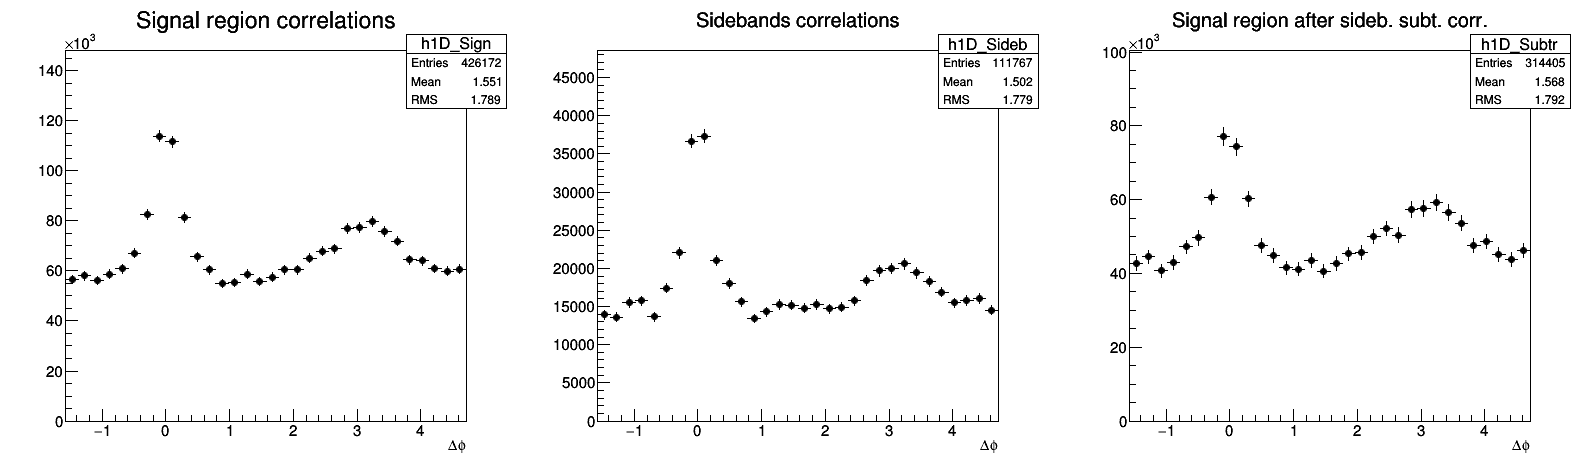
\includegraphics[width=1\linewidth]{{figures/Dzero/h1D_Dzero_Canvas_PtIntBins9to11_PoolInt_thr1dot0to99dot0.png}}
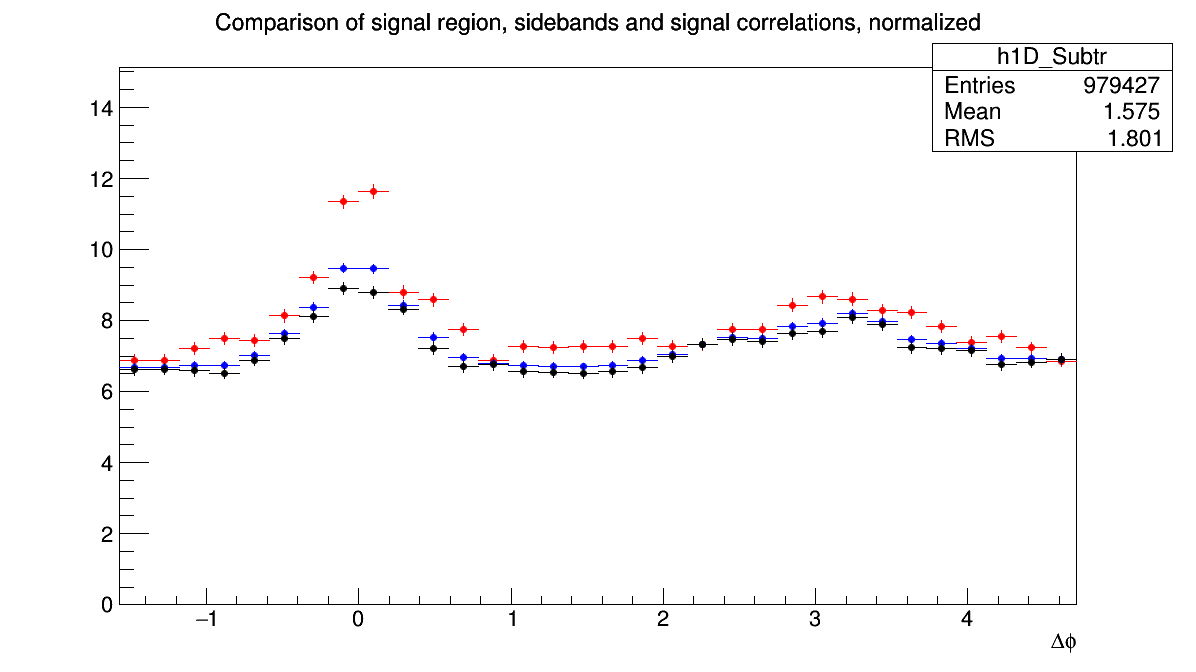
\includegraphics[width=0.8\linewidth]{{figures/Dzero/h1D_Dzero_Canvas_Normalized_PtIntBins9to11_PoolInt_thr0dot3to99dot0.png}}
\caption{Top: Example of $\Dzero$-h signal region (left), sideband (middle), and signal minus sideband (right) correlation distributions. Bottom: signal region per-trigger normalized correlation distribution (blue), sideband region per-trigger normalized correlation distribution (red),
background-subtracted per-trigger normalized correlation distribution (black).}
\label{signReg}
\end{figure}

\item
\underline{\bf Correction for D meson efficiency and associated track efficiency.}
After filling the signal and background correlation distributions, it is necessary to take into account also for the correlations with tracks not reconstructed, or not passing the quality selection due to poor reconstruction. In the same way, the loss of D-mesons which are not reconstructed, or do not pass the selection, impacts the correlation distribution shape. Hence, each pair is weighted by the
inverse of the product of the associated track and D meson reconstruction efficiency, $\epsilon_{trk}$ and $\epsilon_{trig}$. Further details are provided later on in this section.

\item
\underline{\bf Projection in $\Delta\phi$.}
The limited statistics available does not allow to study the two dimensional
$(\Delta\eta,\Delta\phi)$ distribution, which is therefore projected to the $\Delta\phi$ axis by integrating on $|\Delta\eta| <$ 1. Despite, in principle, our maximum $\Delta\eta$ acceptance is of $|\Delta\eta| <$ 1.6, removing the large $|\Delta\eta|$ regions allow us to reject angular regions with very low statistics, where fluctuations would be amplified by a large mixed-event correction, and avoid the so-called wings effect.

As the difference in the azimuthal angle is periodic ($\Delta \phi = 0 = 2\pi$), the $\Delta\phi$-range is limited to the essential range of 2$\pi$. The $\Delta \phi$-limits are chosen to be [$-\pi$/2,3$\pi$/2] in order to provide a good visibility of the correlation pattern, which peaks around 0 and $\pi$.

\item
\underline{\bf Correction for the contamination of secondary particles}
The DCA to primary vertex cut, applied during the associated track selection, has the role of removing the secondary particles from the associated track sample.
Secondary particles are indeed produced either from long-lived strange hadrons or from interaction of particles with the detector material. A residual contamination from secondary tracks is hence expected in the correlation distributions. This contamination is estimated from Monte Carlo simulation
based on Pythia as described more in detail in the next section. The background-subtracted
event-mixing corrected correlations are multiplied by a purity factor to remove this contribution.

\item
\underline{\bf Correction for feed-down of D meson from b-hadron decay}
The selection strategy employed for the D meson candidates selection %to increase the signal over the combinatorial background
enhances the fraction of reconstructed D mesons coming from the decay of a b-hadron. Typical values, with the cuts used for the D-meson selection, are of the order of 10\% or less. The correlation distribution of these secondary D mesons will be sensitive to the properties of beauty jets and beauty hadron decay, which in general differ from those relative to charm jets and hadrons. The procedure used to subtract this contribution is described in the next paragraphs of this section.

\item
\underline{\bf Study of correlation properties.}
The properties of the azimuthal correlation distribution are quantified by
fitting the distribution with a function composed of two Gaussian functions, modelling the near and the away side peaks, and
a constant term describing the baseline. The mean of the Gaussian are fixed at
$\Delta\phi = 0$ and $\Delta\phi = \pi$. To accomplish the $2\pi$ periodicity
of the $\Delta\phi$ variable, the Gaussian functions
are ``duplicated'' with mean at $\Delta\phi = 2\pi$ and $\Delta\phi = -\pi$.
The fitting procedure is described in details in Section \ref{results}.


%The integral of the near side peak and the away side peak
%is dominated by the central parts of the peaks at
%$\Delta \phi = 0$ and $\Delta \phi = \pi$, respectively. Thus, minor
%shape deviations at the side of the peak regions are  acceptable. In
%the following, the fit function is introduced step by step.
%The $\Delta \phi$ distribution can roughly be approximated by a
%constant and two Gaussian functions with the periodicity condition.
%As the $\Delta \phi$-distribution is a periodically continuing
%distribution with $\Delta\phi = 0 = 2\pi$, the fit function has to
%be periodically continuing as well.

\end{enumerate}

\subsection{Mass plots and cut optimization}
The invariant mass distributions in the various $\pt$ ranges studies are shown in Figure~\ref{fig:InvMassD0},~\ref{fig:InvMassDs} and~\ref{fig:InvMassDp} for $\Dzero$, $\Dstar$ and $\Dplus$ respectively.

\begin{figure}[!htp]
\centering

{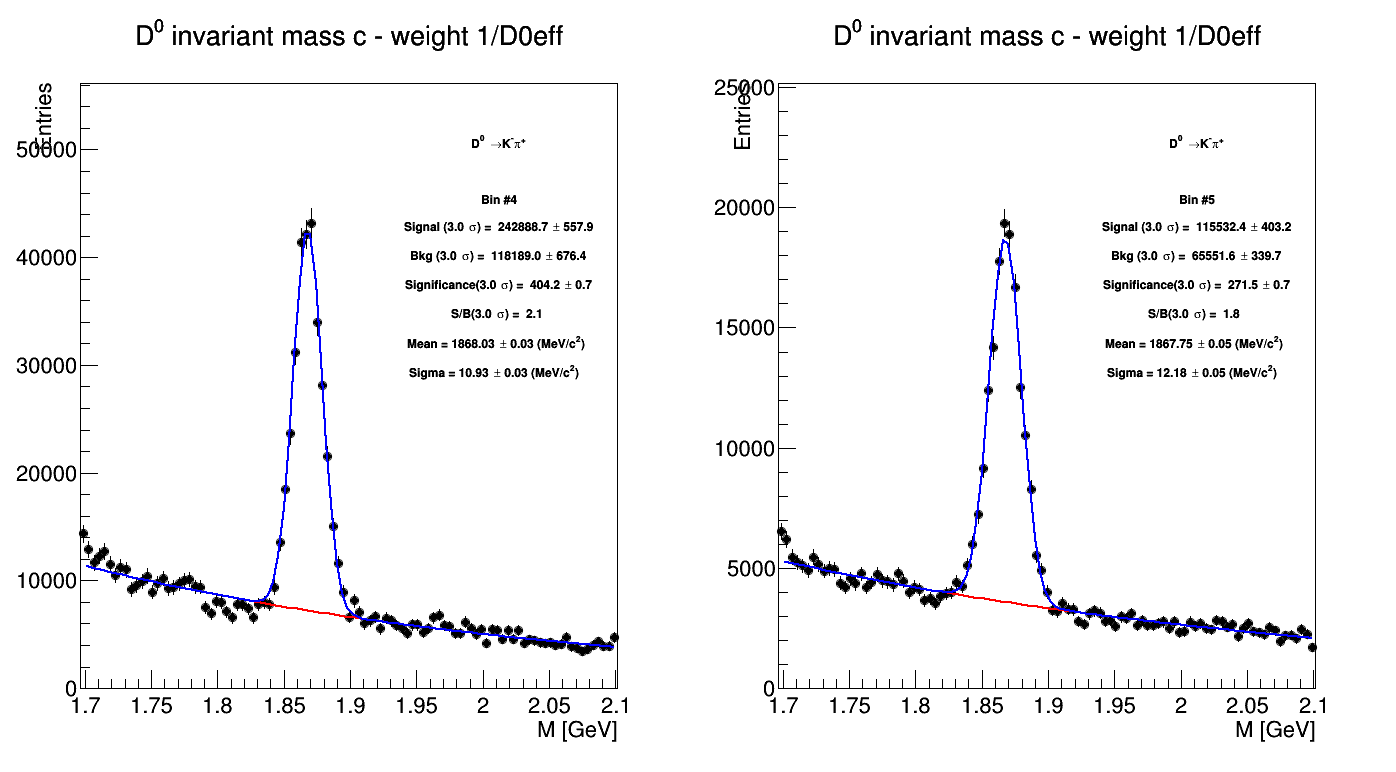
\includegraphics[width=1\linewidth, height=5.6cm]{figures/Dzero/InvMassDistributions_Dzero_Bins4to5.png}}
{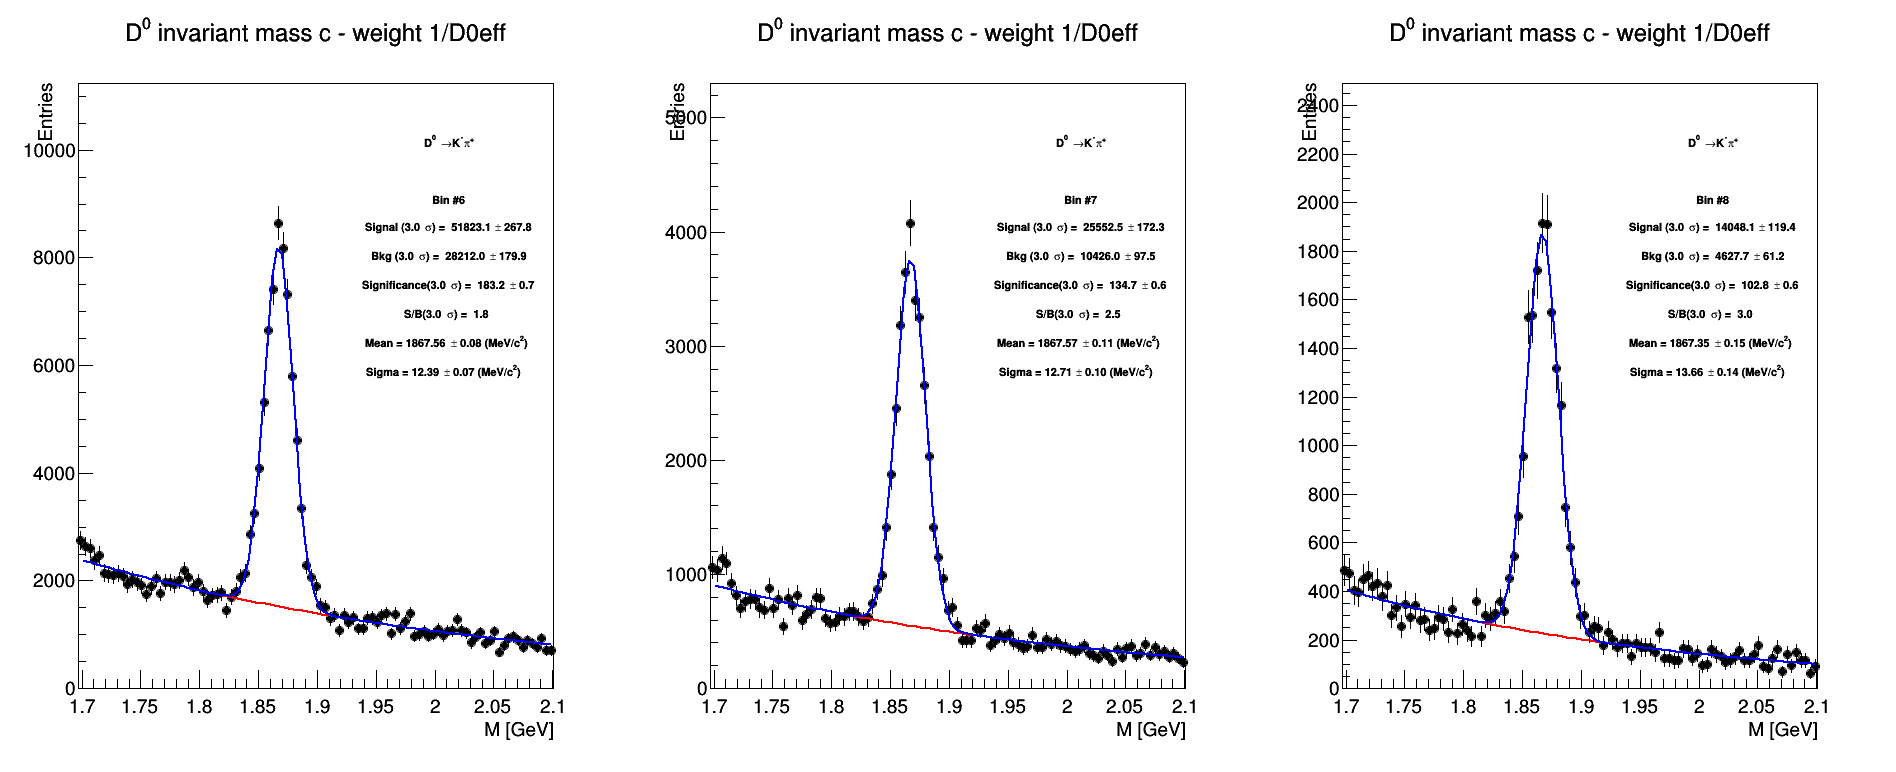
\includegraphics[width=1\linewidth, height=5.6cm]{figures/Dzero/InvMassDistributions_Dzero_Bins6to8.png}}
{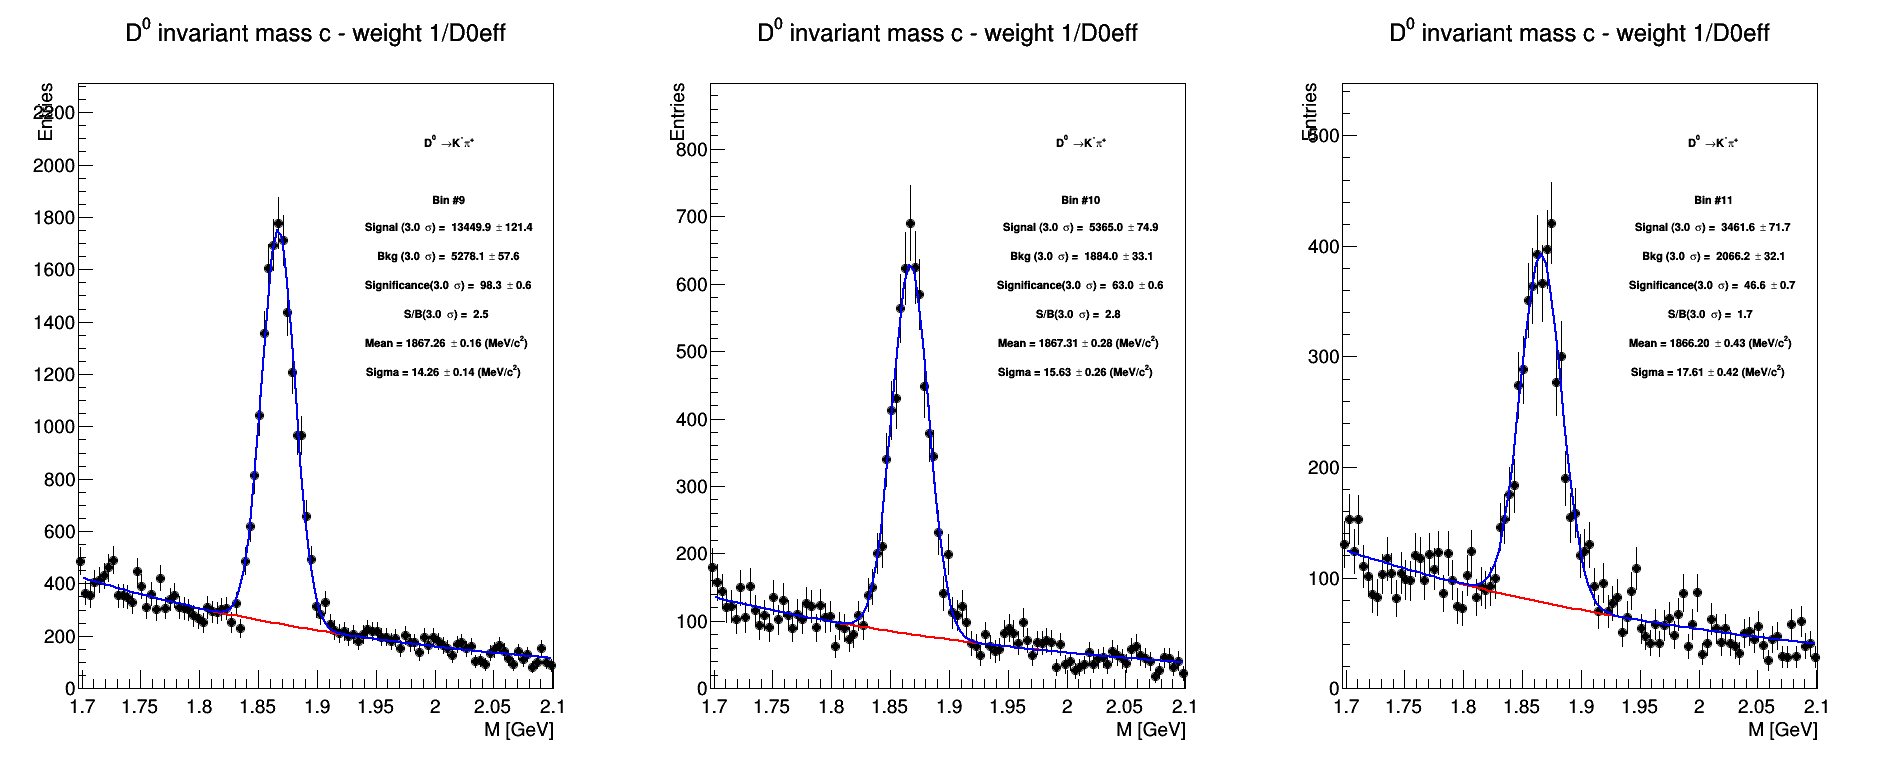
\includegraphics[width=1\linewidth, height=5.6cm]{figures/Dzero/InvMassDistributions_Dzero_Bins9to11.png}}
{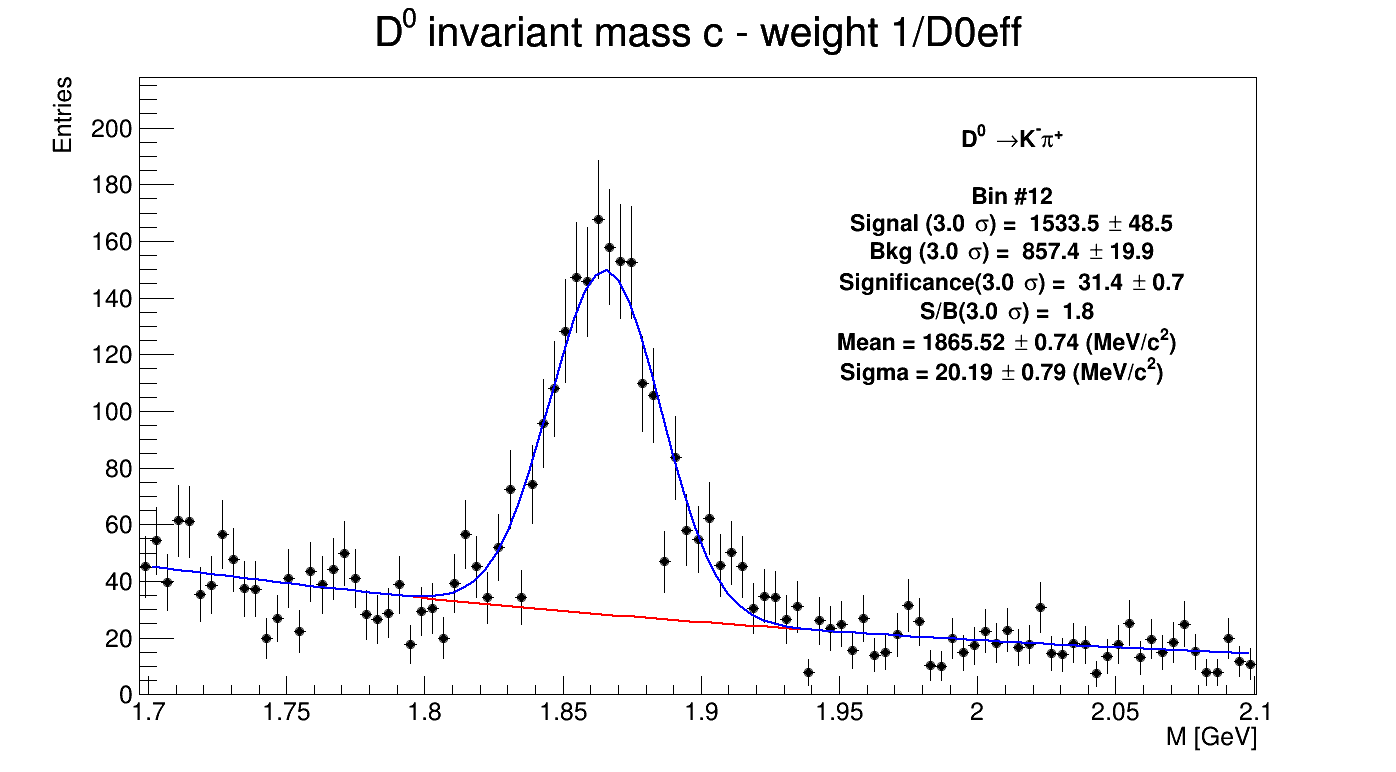
\includegraphics[width=0.6\linewidth, height=5.6cm]{figures/Dzero/InvMassDistributions_Dzero_Bins12to12.png}}

%[width=.32\linewidth]
\caption{Invariant mass distributions of $D^0$ in different $\text{p}_T$ regions. Top: $3< p_{T}^{\text{D}}< 4$ GeV/c (left), $4< p_{T}^{\text{D}}< 5$ GeV/c right), Mid 1: $5< p_{T}^{\text{D}}< 6$ GeV/c (left), $6 < p_{T}^{\text{D}} < 7$ GeV/c (middle), $7< p_{T}^{\text{D}}< 8$ GeV/c (right); Mid2: $8< p_{T}^{\text{D}}< 10$ GeV/c, $10< p_{T}^{\text{D}}< 12$ GeV/c  (middle), $12 < p_{T}^{\text{D}}< 16$ GeV/c  (right) and Bottom: $16<p_{T}^{\text{D}}< 24$ GeV/c.}
\label{fig:InvMassD0}
\end{figure}

\begin{figure}[!htp]
\centering
{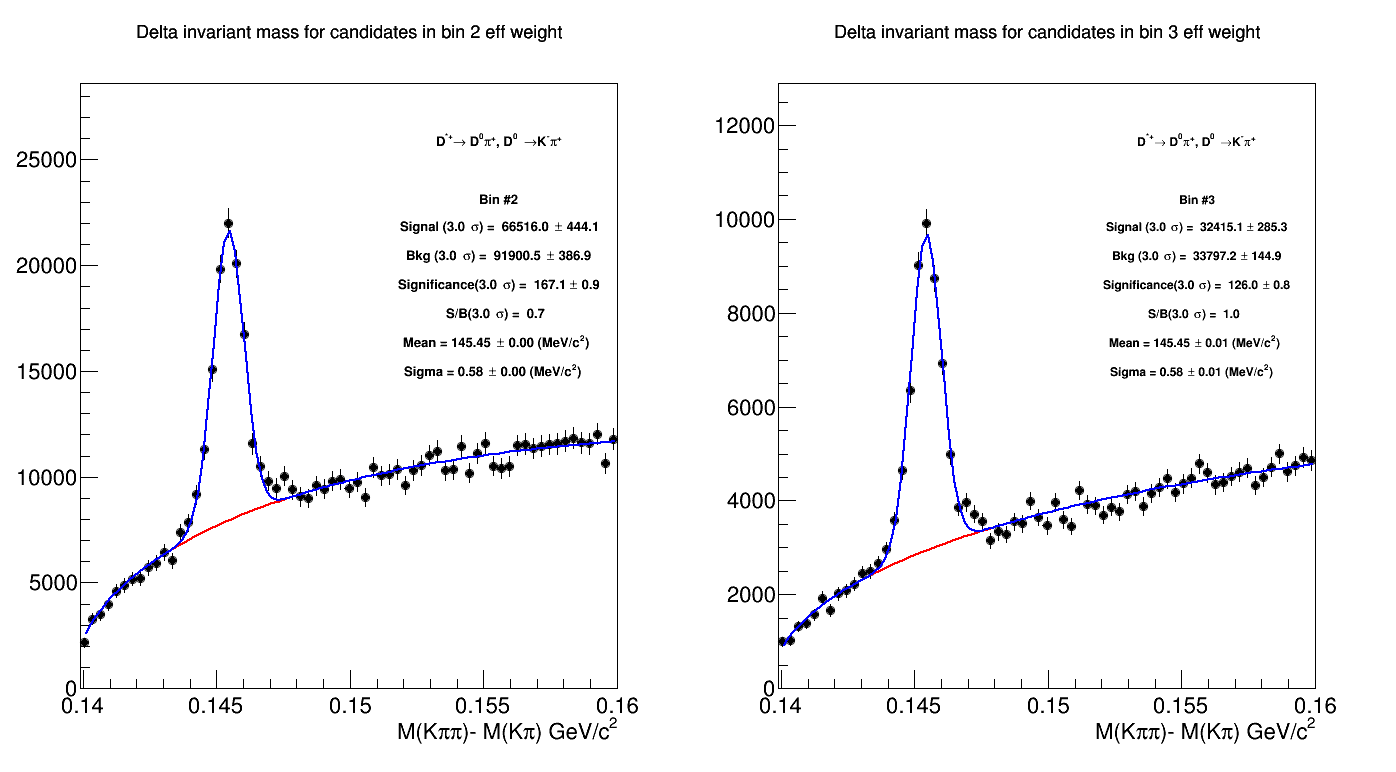
\includegraphics[width=1\linewidth, height=5.6cm]{figures/Dstar_wEFF/InvMassDistributions_Dstar_Bins2to3.png}}
{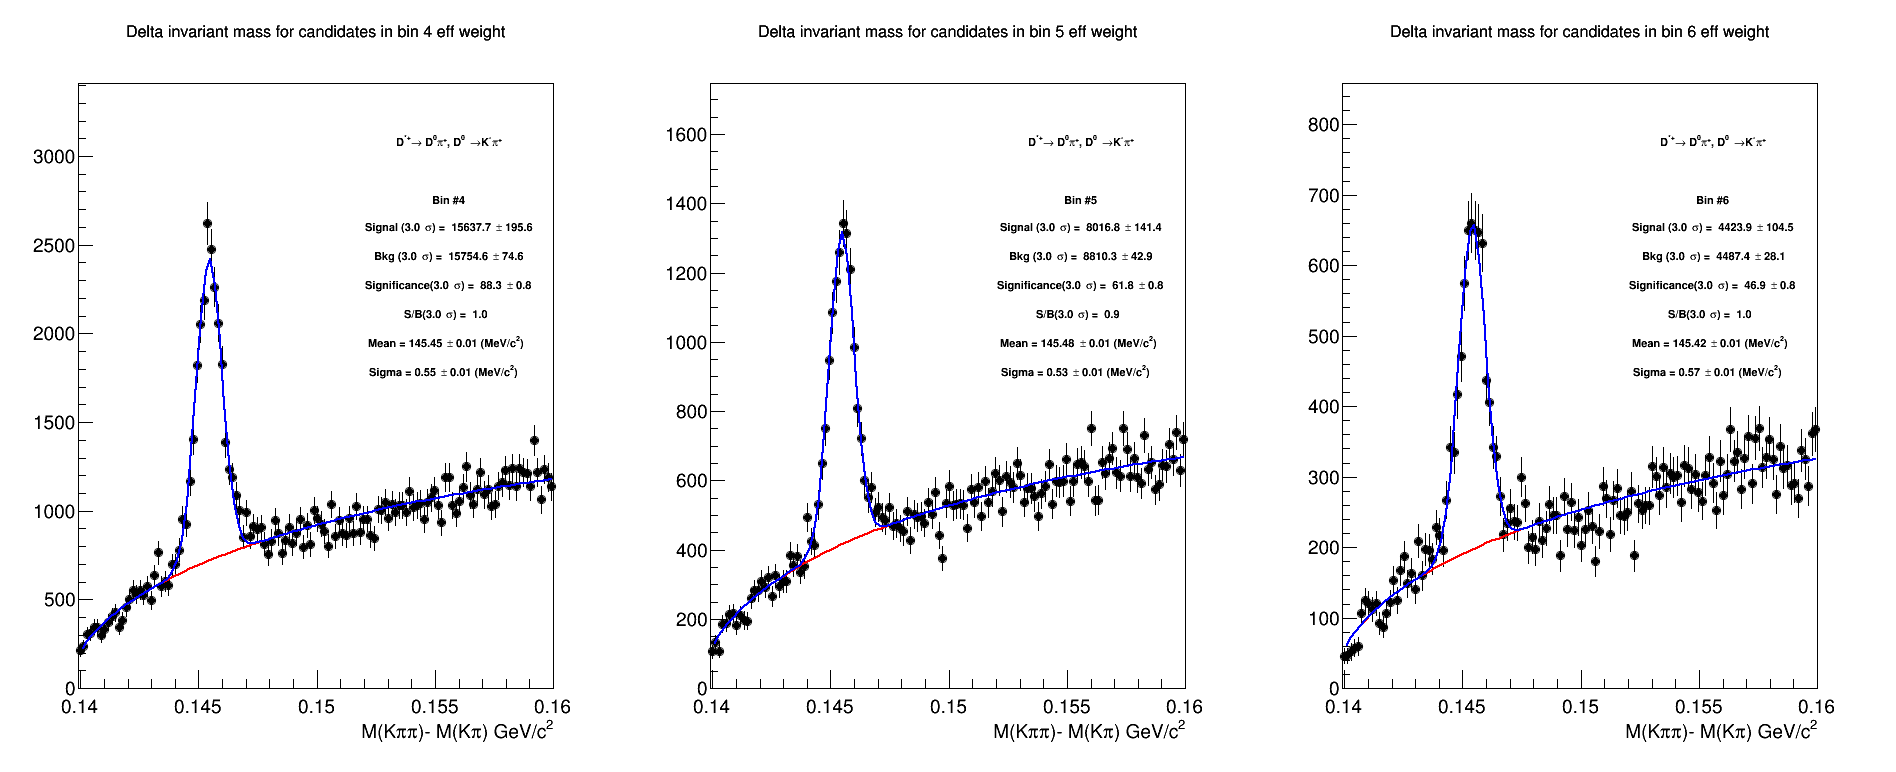
\includegraphics[width=1\linewidth, height=5.6cm]{figures/Dstar_wEFF/InvMassDistributions_Dstar_Bins4to6.png}}
{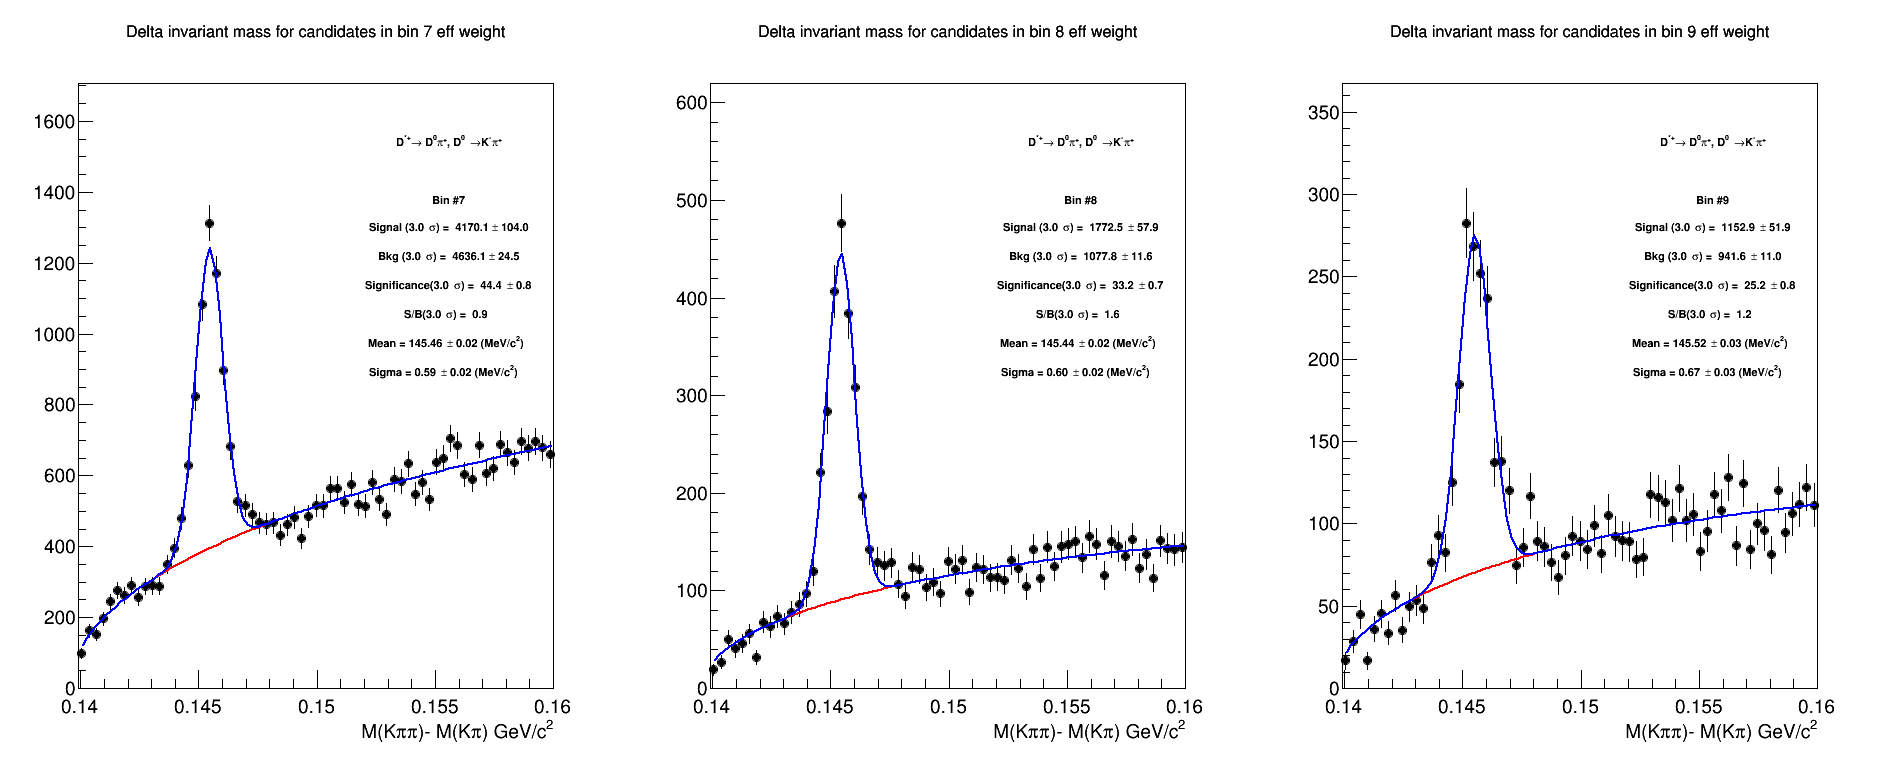
\includegraphics[width=1\linewidth, height=5.6cm]{figures/Dstar_wEFF/InvMassDistributions_Dstar_Bins7to9.png}}
{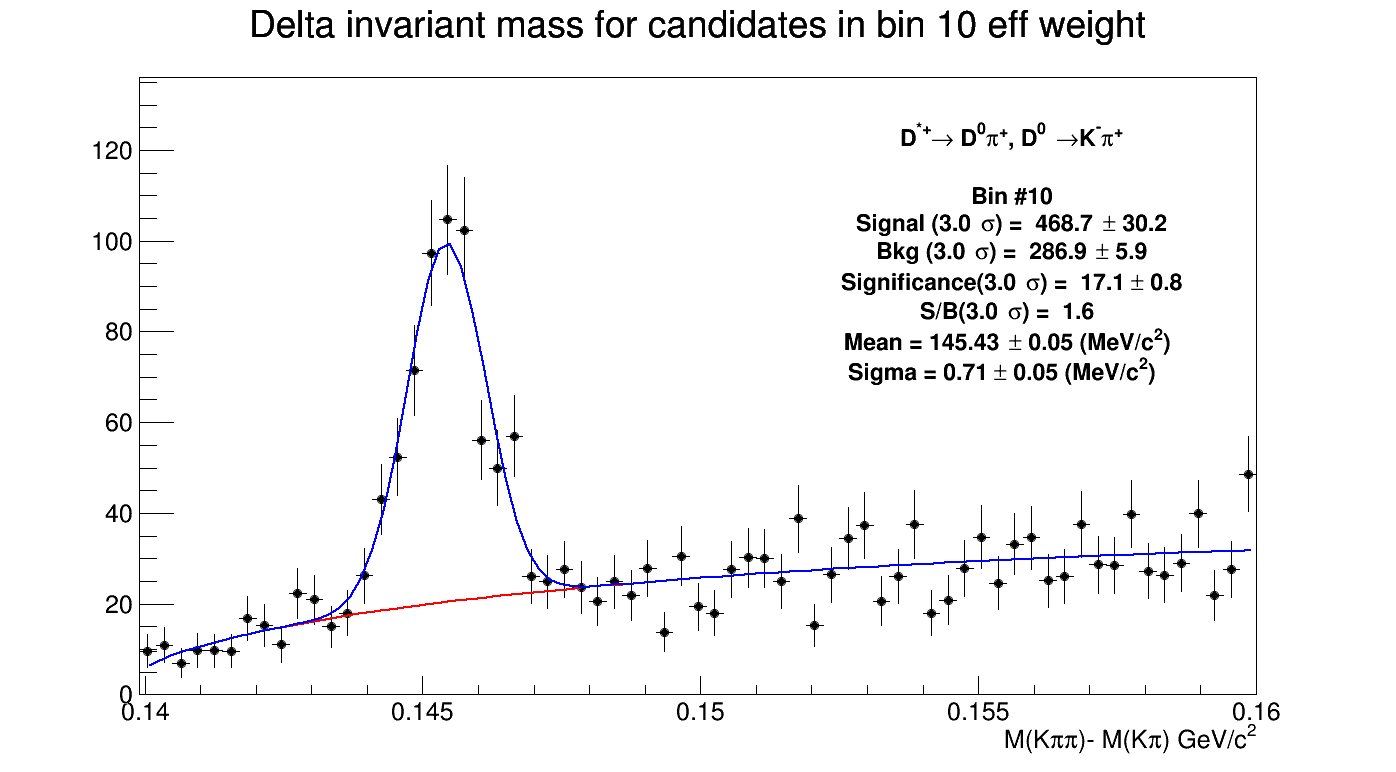
\includegraphics[width=0.6\linewidth, height=5.6cm]{figures/Dstar_wEFF/InvMassDistributions_Dstar_Bins10to10.png}}

\caption{Invariant mass distributions of $\Dstar$ in different $\text{p}_T$ regions. Top: $3< p_{T}^{\text{D}}< 4$ GeV/c (left), $4< p_{T}^{\text{D}}< 5$ GeV/c right), Mid 1: $5< p_{T}^{\text{D}}< 6$ GeV/c (left), $6 < p_{T}^{\text{D}} < 7$ GeV/c (middle), $7< p_{T}^{\text{D}}< 8$ GeV/c (right); Mid2: $8< p_{T}^{\text{D}}< 10$ GeV/c, $10< p_{T}^{\text{D}}< 12$ GeV/c  (middle), $12 < p_{T}^{\text{D}}< 16$ GeV/c  (right) and Bottom: $16<p_{T}^{\text{D}}< 24$ GeV/c .}
\label{fig:InvMassDs}
\end{figure}

\begin{figure}[!htp]
\centering
{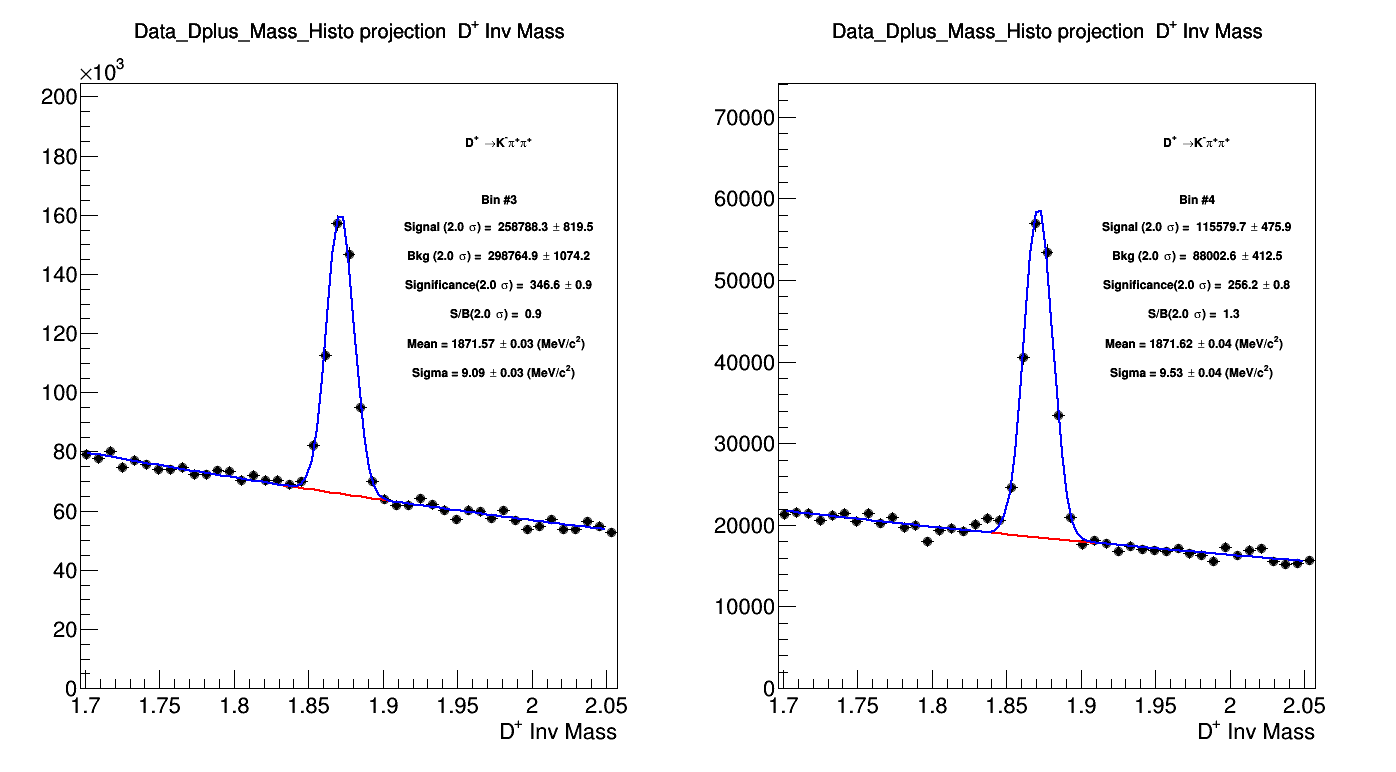
\includegraphics[width=1\linewidth, height=5.6cm]{figures/DplusPlotsweff/InvMassDistributions_Dplus_Bins3to4.png}}
{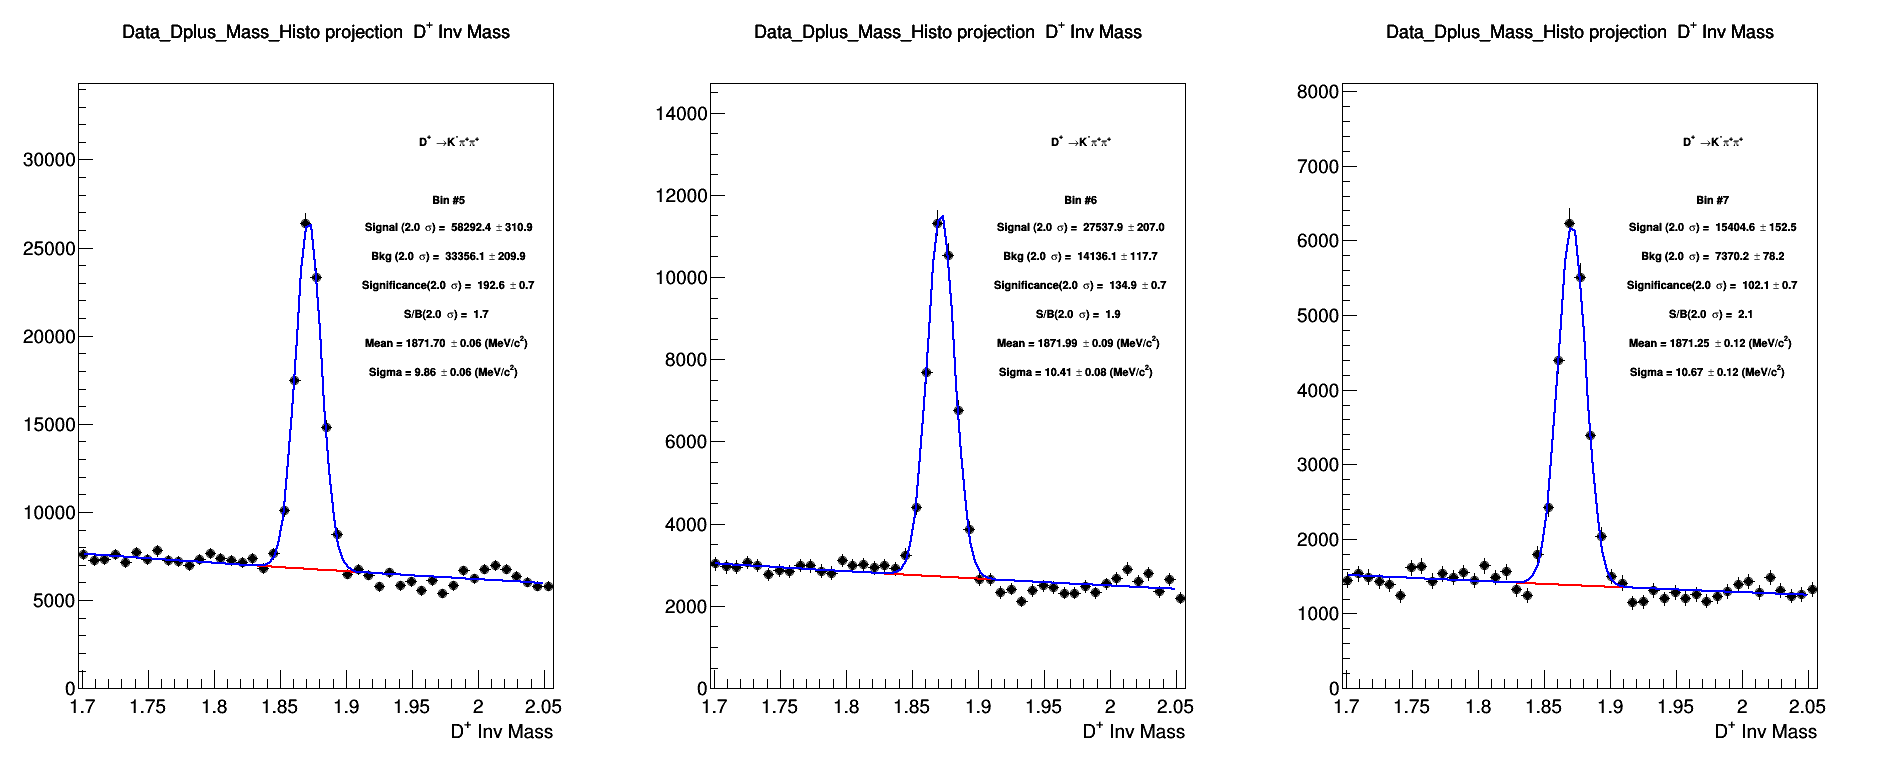
\includegraphics[width=1\linewidth, height=5.6cm]{figures/DplusPlotsweff/InvMassDistributions_Dplus_Bins5to7.png}}
{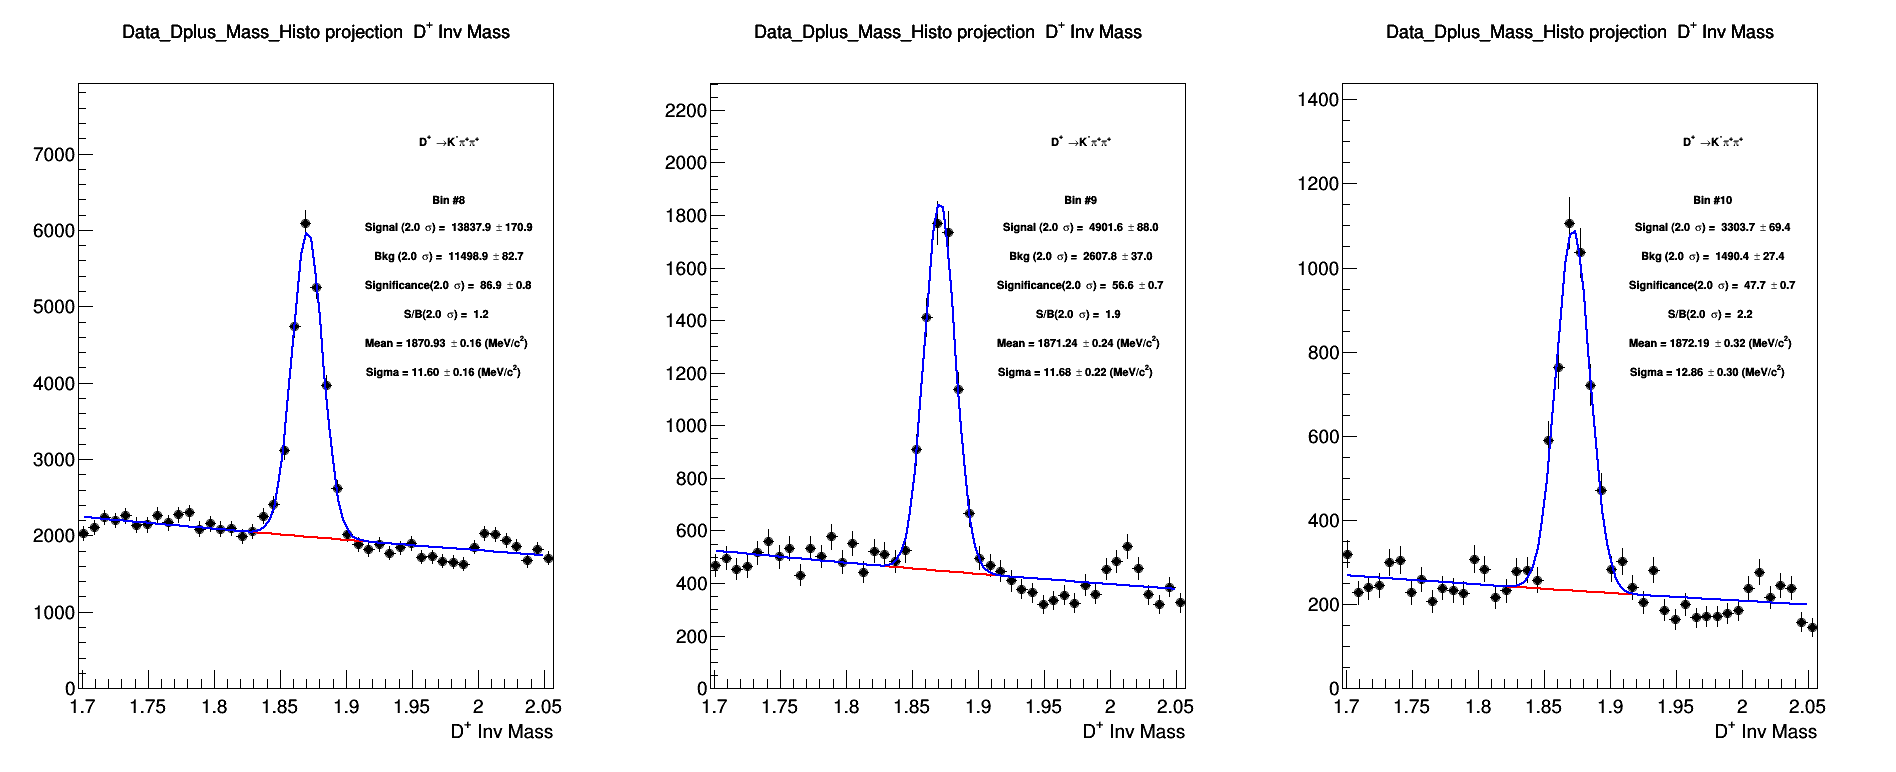
\includegraphics[width=1\linewidth, height=5.6cm]{figures/DplusPlotsweff/InvMassDistributions_Dplus_Bins8to10.png}}
{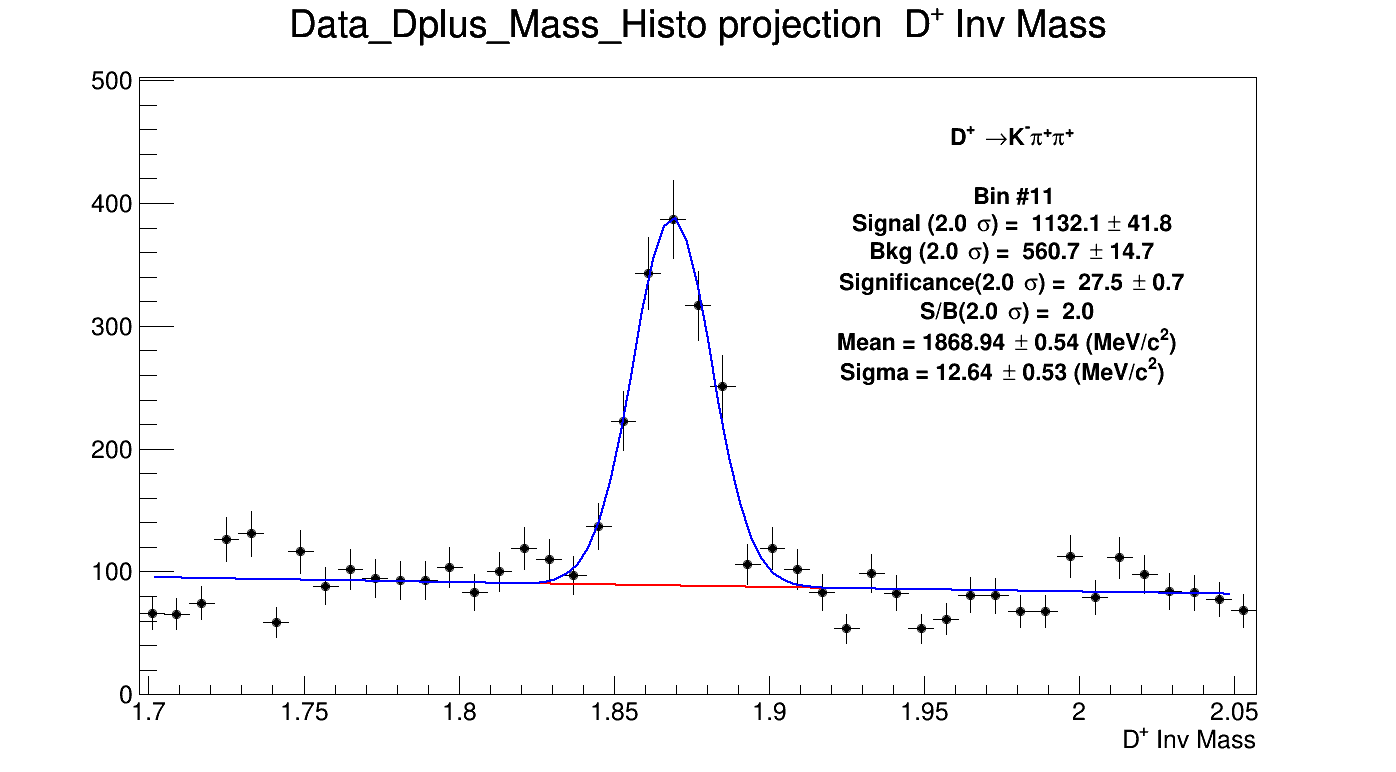
\includegraphics[width=0.6\linewidth, height=5.6cm]{figures/DplusPlotsweff/InvMassDistributions_Dplus_Bins11to11.png}}

\caption{Invariant mass distribution of $\Dplus$ in different $\text{p}_T$ regions. Top: $3< p_{T}^{\text{D}}< 4$ GeV/c (left), $4< p_{T}^{\text{D}}< 5$ GeV/c right), Mid 1: $5< p_{T}^{\text{D}}< 6$ GeV/c (left), $6 < p_{T}^{\text{D}} < 7$ GeV/c (middle), $7< p_{T}^{\text{D}}< 8$ GeV/c (right); Mid2: $8< p_{T}^{\text{D}}< 10$ GeV/c, $10< p_{T}^{\text{D}}< 12$ GeV/c  (middle), $12 < p_{T}^{\text{D}}< 16$ GeV/c  (right) and Bottom: $16<p_{T}^{\text{D}}< 24$ GeV/c .}
\label{fig:InvMassDp}
\end{figure}

For $\Dstar$, the standard D2H p-Pb cuts (for the 2013 cross section analysis) were used. The same holds for the $\Dplus$, but with the addition of cuts on the normalized decay length in $xy$ plane and of the normalized difference between measured and expected daughter track impact parameters (topomatic cut).
A particular cut optimization was instead performed for the $\Dzero$ meson. Twelve cut sets were tried, with the goal of increasing the S/B factor, in order to reduce fluctuations induced by the sideband subraction (the limiting factor for the analysis performance).
In Figure \ref{fig:cutoptD0} the $\Dzero$-h correlation distributions are shown for the different cut sets, in exemplary kinematic regions (left column), together with the bin-by-bin relative statistical uncertainty on the data points (right column). The best cut set (option G) was defined from the standard cuts used for the p-Pb 2013 cross section analysis, with a tightened selection on the cosine of the pointing angle, and with the addition of a cut on the normalized decay length in $xy$ plane and of a selection on the normalized difference between measured and expected daughter track impact parameters (topomatic cut).

\begin{figure}[!htp]
\centering
{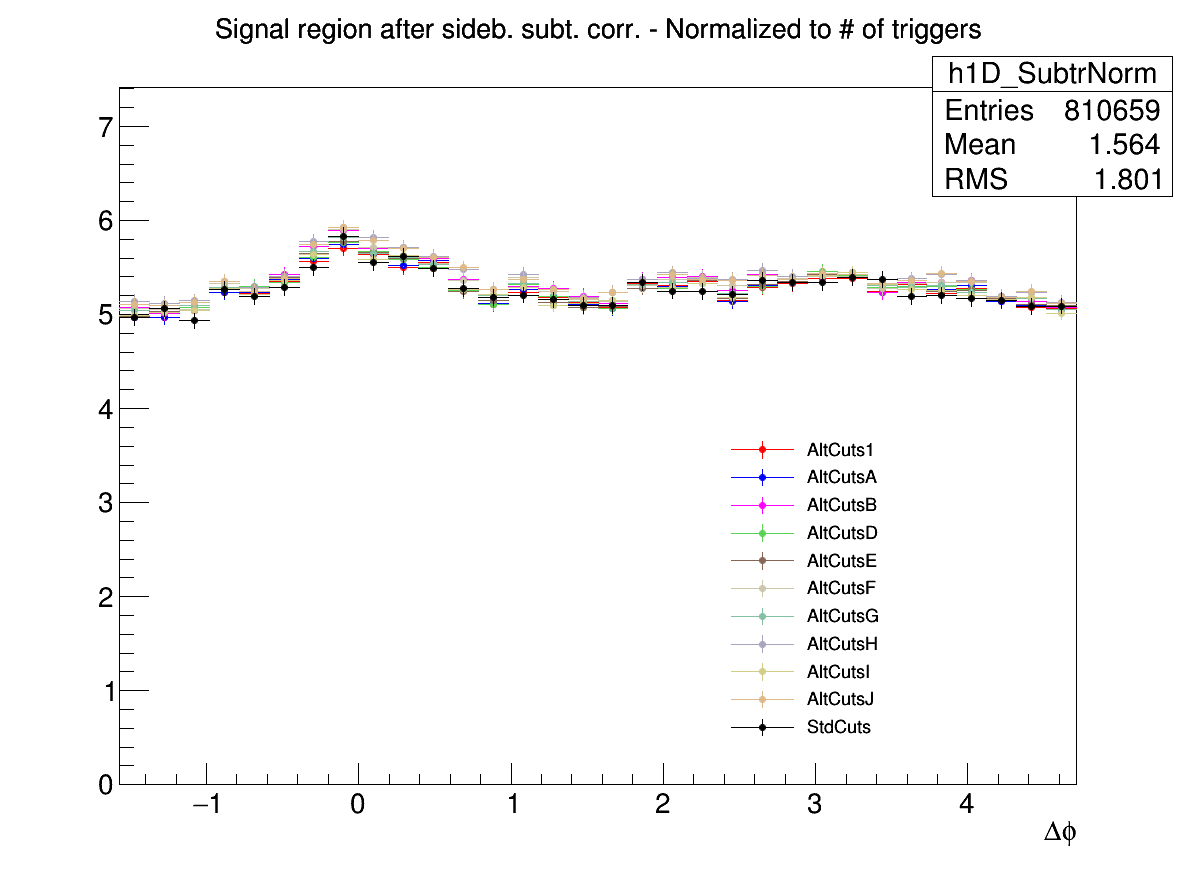
\includegraphics[width=0.47\linewidth, height=5.6cm]{figures/Cut_Optimiz_D0/AzimCorrDistr_Dzero_Canvas_PtIntBins3to5_PoolInt_thr03to99_Superimp.png}}
{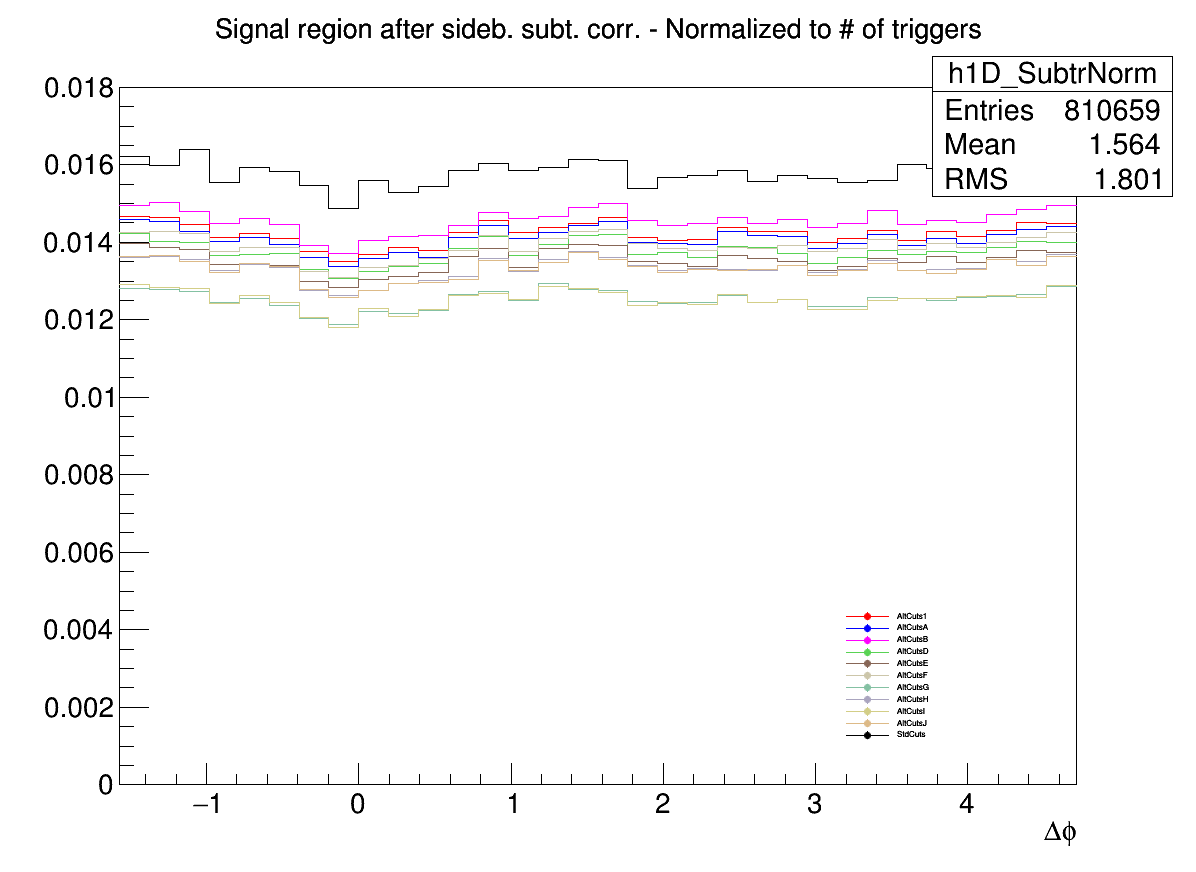
\includegraphics[width=0.47\linewidth, height=5.6cm]{figures/Cut_Optimiz_D0/Uncertanty_AzimCorrDistr_Dzero_Canvas_PtIntBins3to5_PoolInt_thr03to99.png}}
{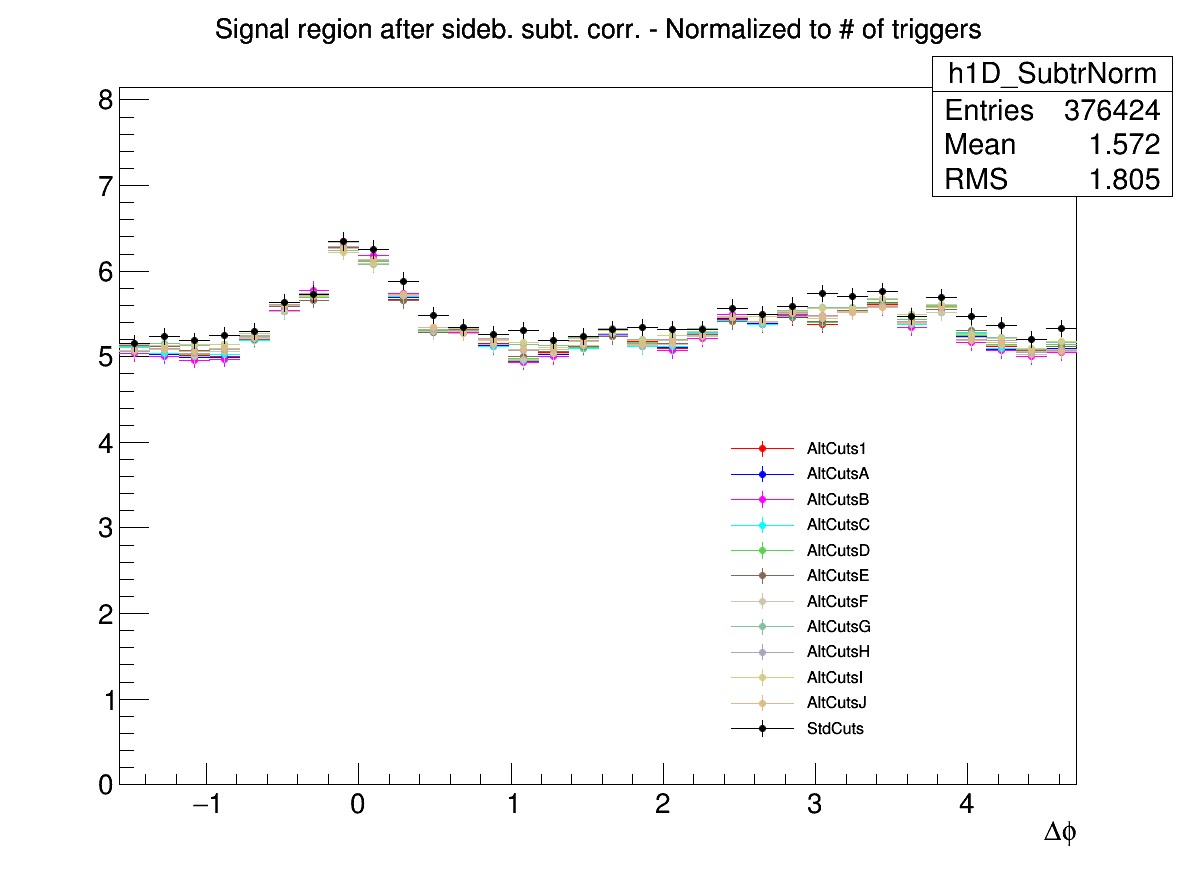
\includegraphics[width=0.47\linewidth, height=5.6cm]{figures/Cut_Optimiz_D0/AzimCorrDistr_Dzero_Canvas_PtIntBins6to8_PoolInt_thr03to99_Superimp.png}}
{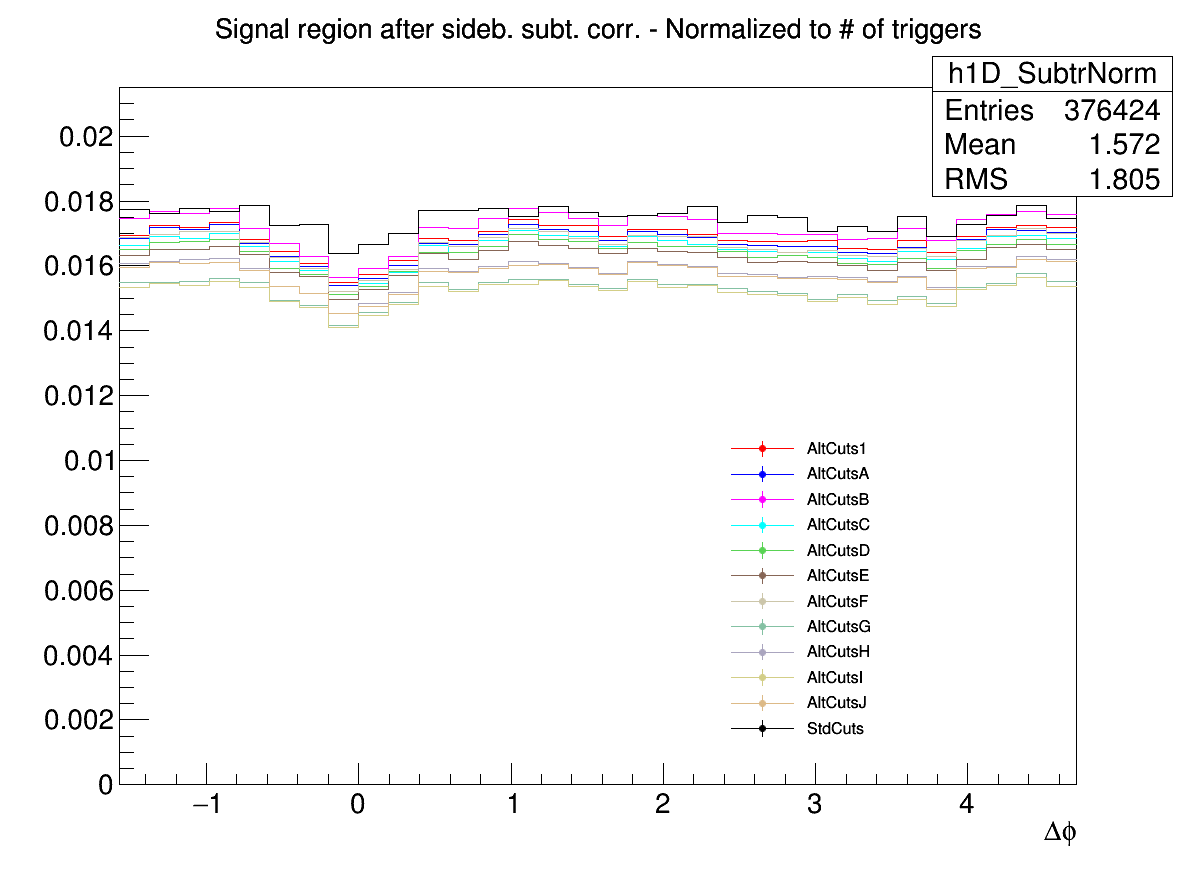
\includegraphics[width=0.47\linewidth, height=5.6cm]{figures/Cut_Optimiz_D0/Uncertanty_AzimCorrDistr_Dzero_Canvas_PtIntBins6to8_PoolInt_thr03to99.png}}
{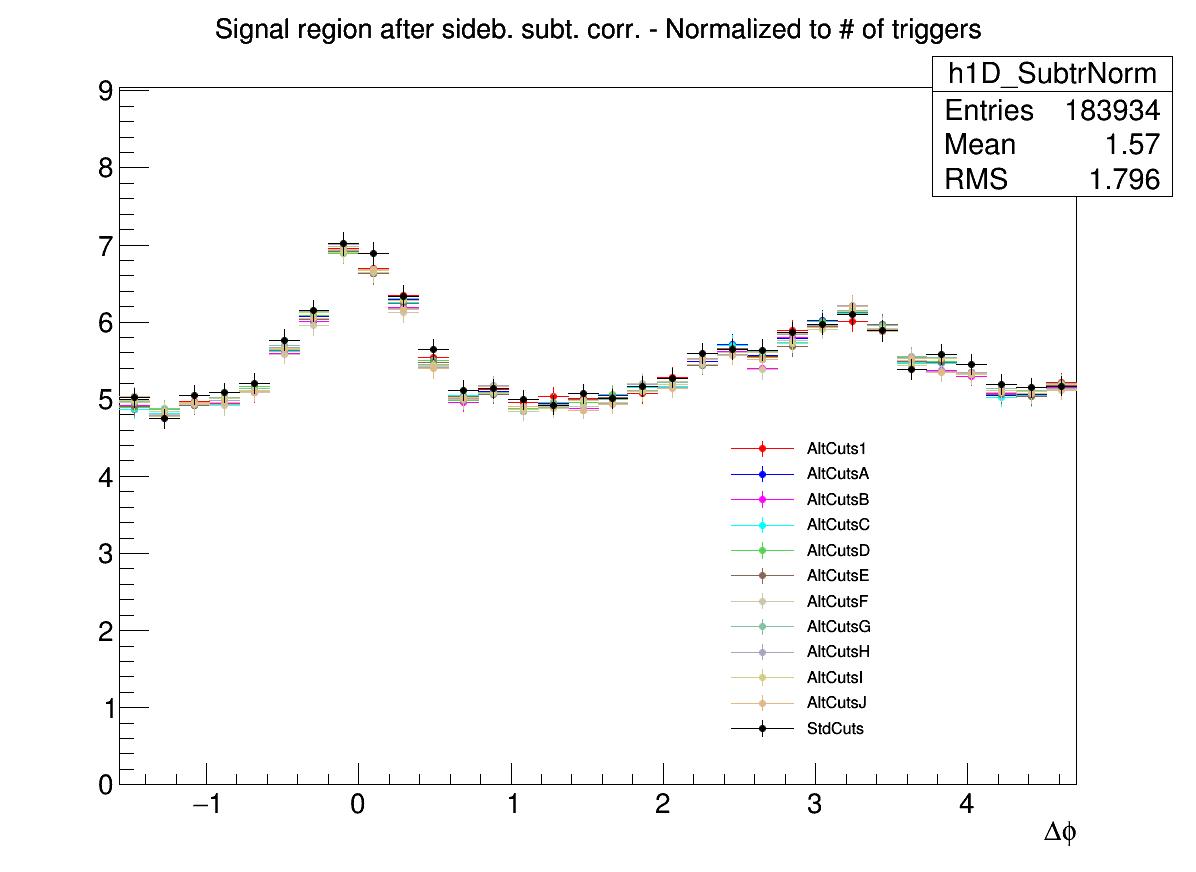
\includegraphics[width=0.47\linewidth, height=5.6cm]{figures/Cut_Optimiz_D0/AzimCorrDistr_Dzero_Canvas_PtIntBins9to10_PoolInt_thr03to99_Superimp.png}}
{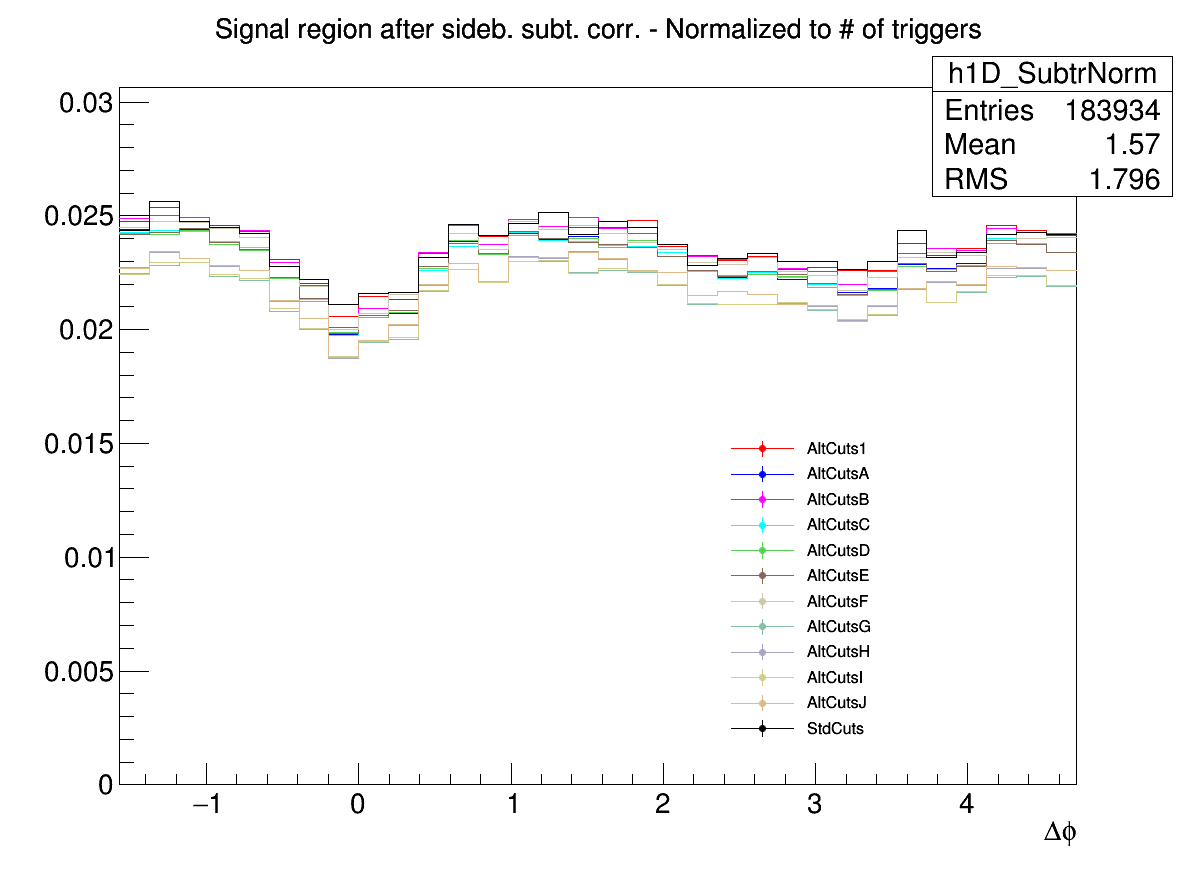
\includegraphics[width=0.47\linewidth, height=5.6cm]{figures/Cut_Optimiz_D0/Uncertanty_AzimCorrDistr_Dzero_Canvas_PtIntBins9to10_PoolInt_thr03to99.png}}

\caption{$\Dzero$-h correlation distributions with different cut options (left) and point-by-point relative statistical uncertainty (right) for $3< p_{T}^{\text{D}}< 5$ GeV/c (top), $5< p_{T}^{\text{D}}< 8$ GeV/c (middle), $8< p_{T}^{\text{D}}< 16$ GeV/c (bottom), in all cases with associated track $\pt$ $> 0.3$ GeV/c.}
\label{fig:cutoptD0}
\end{figure}

\subsection{Code used for the analysis}
The code used for D meson-hadron correlation analysis is fully committed in AliPhysics. The analysis classes can be found in
\$ALICE\_ROOT/PWGHF/correlationHF/.  The  D meson specific classes where the aforementioned steps are carried out are
AliAnalysisTaskDStarCorrelations, AliAnalysisTaskSED0Correlations and AliAnalysisTaskDplusCorrelations. The classes which are common to the D meson specific analysis which includes the associated particle cuts and the correlation observables are AliHFAssociatedTrackCuts, AliHFCorrelator, AliHFOfflineCorrelator, AliReducedParticle and AliDhCorrelationExtraction. Several additional classes and macros in the same folder deal with the correction steps.

\subsection{Further details on corrections}
\subsubsection{Event Mixing}
The event-mixing technique is used for correcting the raw correlation distribution for effects arising
from the detector limited acceptance in rapidity and detector spatial inhomogeneities. The calculation of the Event
Mixing correlation distribution is performed online.%, following the strategy and the code developed for the \textit{PWGCF} correlation analyses. 
An event pool is created, where events preceding the one containing a D candidate are stored based on their properties (position of the vertex along the z axis and multiplicity). 
Each time a D meson candidate is found in an event, only the events contained in the same pool as the event under analysis is used to evaluate the correlations for the event mixing correction.% the correlation analysis on the mixed events is performed if the pool satisfies the conditions defined at its creation, being the same as described for the pp analysis (As well as the conditions for refreshing the pools).

The multiplicity and z vertex position bins for the pools used in the p-Pb analysis are the following:
\begin{itemize}
\item Multiplicity bins: $\left(0,40\right);\left(40,65\right);\left(65,+\infty\right)$
\item Vertex z $(cm)$ = $\left(-10,-2.5\right);\left(-2.5,2.5\right);\left(2.5,10\right)$
\end{itemize}
%(\ref{tab:em})


In an ideal case, the mixed event distribution is expected to have a constant flat distribution as function of $\Delta\phi$ and a triangular shaped distribution in $\Delta\eta$
deriving from the limited $\eta$ acceptance of the detector. The obtained distribution is used as a weight in each correlation bin, i.e, the corrected correlation distribution is calculated as follows:
\begin{equation}
\label{eq:mixing}
\frac{dN^{corr}\left(\Delta\phi \Delta\eta\right)}{d\Delta\phi d\Delta\eta} = \frac{\frac{dN^{SE}\left(\Delta\phi \Delta\eta\right)}{d\Delta\phi d\Delta\eta} }{\frac{dN^{ME}\left(\Delta\phi \Delta\eta\right)}{d\Delta\phi d\Delta\eta} }\frac{dN^{ME}\left(0,  0\right)}{d\Delta\phi d\Delta\eta}
\end{equation}
In the previous equation, the last term stands for the average of the bins in the region $-0.2 < \Delta\eta < 0.2$, $-0.2 < \Delta\phi < 0.2$ (multiple bins are used to minimize the effect of statistical fluctuations on the normalization of the mixed-event plots).

The mixed-event correlation distributions are built in both D meson signal and sideband regions. Both are
corrected with the relative distributions. An example of the mixed event distribution is shown in Fig.~\ref{fig:DplusSEbyMEPlots1} (middle panels). The expected triangular
shape in $\Delta\eta$ addresses the effect of the limited detector pseudo-rapidity acceptance. Note that the mixed-event distribution is limited to
the interval $\left|\Delta\eta\right|<1$: the decision to limit the mixed-event correction, and thus the whole analysis, to this range was taken in
order to avoid the so-called ``wing effect", i.e. the wing-like structures arising in the correlation distribution at large $\Delta\eta$ due to the
limited filling of the correlation bins in that region. The event mixing is calculated in the \textit{AliHFCorrelator} class and is computed in the same way for each D meson.


\begin{comment}
\begin{figure}[!ht]
\centering
%{\includegraphics[width=.95\linewidth]{figures/Dplus_low_dot5_SEbyME.png}}
 \caption{($\Delta \phi , \Delta \eta$) correlation in the Sidebands and Signal region from Single Event and Mixing Event analysis for low $p_{T}$: $3 < p_{T}^{\text{D}^+} < 5 GeV/c$ with associated track $p_{T}$ threshold 0.3 GeV/c }
\label{fig:DplusSEbyMEPlots1}
\end{figure}



\begin{figure}[!ht]
\centering
%Marianna
%{\includegraphics[width=.95\linewidth]{figures/Dplus_mid_dot5_SEbyME.png}}
 \caption{($\Delta \phi , \Delta \eta$) correlation in the Sidebands and Signal region from Single Event and Mixing Event analysis for mid $p_{T}$: $5< p_{T}^{\text{D}^+}< 8 GeV/c$ with associated track $p_{T}$ threshold 0.3 GeV/c }
\label{fig:DplusSEbyMEPlots2}
\end{figure}

\begin{figure}[!ht]
\centering
%{\includegraphics[width=.95\linewidth]{figures/Dplus_high_dot5_SEbyME.png}}
 \caption{($\Delta \phi , \Delta \eta$) correlation in the Sidebands and Signal region from Single Event and Mixing Event analysis for high $p_{T}$: $8< p_{T}^{\text{D}^+}< 16 GeV/c$ with associcated track $p_{T}$ threshold 0.3 GeV/c }
\label{fig:DplusSEbyMEPlots3}
\end{figure}

Figures \ref{fig:DplusSEbyMEPlots1}, \ref{fig:DplusSEbyMEPlots2}, \ref{fig:DplusSEbyMEPlots3} show the 2D correlation in Sideband Region and Signal region from SE and ME analysis for $D^+$ meson in different $p_{T}$ region.

\end{comment}

\newpage
\subsubsection{Tracking and D-meson trigger efficiency}

{\bf \normalsize (i) Tracking efficiency}: is calculated by obtaining the ratio between the yield at the reconstructed level and generated level, for a defined ``type" of particles (in our case non-identified particles) and it is estimated differentially in p$_T$, $\eta$, and z$_{vtx}$ of the event.\\
{\bf Implementation }: tracking efficiency maps are produced as TH3D histograms (p$_T$, $\eta$, z$_{vtx}$) obtained from MC analysis on the minimum-bias samples LHC17a2b$\_$fast and LHC17a2b$\_$cent$\_$woSDD, and applying at reconstructed level the track selections (summarized in Table.~\ref{table:effCuts}). These efficiency maps are used in the analysis tasks to extract single track efficiencies; each correlation pairs found in the data analysis is inserted in correlation plots with a weight of {\bf 1/efficiency value}. Example plots of the tracking efficiencies as a function of p$_T$ are shown in Fig.~\ref{fig:trackeff}.


%\begin{figure}[h]
%	\centering
%	\includegraphics[scale=0.35]{figures/pPb_STE_1D_pT_all_DCA.png}
%	\caption{Charged particle $p_T$ efficiency for different DCA values.}
%	\label{fig:trackeff}	
%\end{figure}


\begin{figure}[h]
	\centering
	%\includegraphics[scale=0.35]{figures/pPb_efficiencyVsspeicies.png}
	\caption{$p_T$ efficiency for standard track selection.}
	\label{fig:trackeffvsspecies}	
\end{figure}

\newpage
Details of cuts at event level and particle selection at different steps are listed in Table.~\ref{table:effCuts} . \\
\begin{table}[h]
\small
\centering % used for centering table

\begin{tabular}{  p{5cm} |  p{8.5cm} }
 \\
  \multirow{1}{*}{\large \textbf {MC Generated }} \\
\hline
\\
     Stages         &              Cuts \\
\hline\hline & \\		            	
  1.MC Part with Generated Cuts         &    {\textbf {After Event Selection}}\\
																		   & Charge\\
																		    & PDG Code\\
														  				  & Physical Primary \\

   2. MC Part with Kine Cuts         &              {\textbf {Kinematics Cuts }}\\
															    & -0.8$\textless \eta \textless  0.8$\\
															    & pT $\textgreater$ 0.3 (GeV/$c$)\\

&		\\            	


\multirow{1}{*}{\large \textbf {MC Reconstructed }} & \\
\hline


\hline & \\		            	                        	
4. Reco tracks        &                             {\textbf {After Event Selection}}\\
															   & Physical Primary \\
															
															
5. Reco tracks with Kine Cuts         &               {\textbf  {Kinematics Cuts }}\\
															    & -0.8$\textless \eta \textless  0.8$\\
															    & pT $\textgreater$ 0.3 (GeV/$c$)\\



6. MC true with Quality Cuts         &      			      {\textbf  {Quality Cuts }} \\
																	&SetRequireSigmaToVertex(kFALSE) \\
																	&SetDCAToVertex2D(kFALSE) \\
																	&SetMinNCrossedRowsTPC(70)\\
																	&SetMinRatioCrossedRowsOverFindableClustersTPC(0.8)\\
																	&SetMinNClustersITS(3)\\
																	&SetMaxChi2PerClusterTPC(4)\\
																	&SetMaxDCAToVertexZ(1) \\
																	&SetMaxDCAToVertexXY(0.25) \\
																	&SetRequireTPCRefit(TRUE) \\
																	&SetRequireITSRefit(FALSE) \\

7. Reco tracks with Quality Cuts         &             {\textbf  {Same as step 6}} \\

 &\\		            	            		

 \hline \hline
 \\
\end{tabular}
\caption{\large {Single Track Efficiency cuts detail}} % title of Table
\label{table:effCuts}	
\end{table}


{\bf \large (ii) D Meson efficiency} - Due to limited statistics, the correlation analysis is performed in quite wide p$_\mathrm{T}$ bins and in each of them the reconstruction and selection efficiency of D mesons is not flat (Fig.~\ref{fig:dpluseff},~\ref{fig:d0eff}), in particular in the lower $\pt$ region. We correct for the p$_\mathrm{T}$ dependence of the trigger efficiency within each p$_\mathrm{T}$-bin.
This correction is applied online, by using a map of D meson efficiency as a function of p$_\mathrm{T}$ and event multiplicity (in terms of SPD tracklets in $|\eta|<1$) extracted from the enriched Monte Carlo sample LHC17d2a$\_$fast$\_$new.
While running the analysis, each correlation entry is weighted by {\bf 1/trigger efficiency}. It was observed that multiplicity dependence of the efficiency does not bias the extraction of the signal yield from the invariant mass distributions (which, as anticipated, are also weighted in the same manner). Efficiency plots for $\Dzero$, $\Dplus$ and $\Dstar$ mesons are shown in Fig.~\ref{fig:doeff}, Fig.~\ref{fig:dpluseff} and ~\ref{fig:dstareff}.

\begin{figure}[!htp]
	\centering
%Marianna
	%\includegraphics[width=.48\linewidth]{figures/D0Eff_From_c_wLimAcc_2D_pPb.png}  % by Fabio
	%\includegraphics[width=.48\linewidth]{figures/D0Eff_From_c_wLimAcc_1D_pPb.png} \\
	%\includegraphics[width=.30\linewidth]{figures/D0Eff_ProjMult_3to4GeV.png}
	%\includegraphics[width=.30\linewidth]{figures/D0Eff_ProjMult_5to6GeV.png}
	%\includegraphics[width=.30\linewidth]{figures/D0Eff_ProjMult_8to12GeV.png}
\caption{Top panel: (p$_\mathrm{T}$, multiplicity) dependence (left) and p$_T$ dependence (right) of prompt $D^0$ meson efficiency. Bottom panels: multiplicity dependence of $D^0$ meson efficiency for three $D^0$ p$_\mathrm{T}$ ranges: 3-4 GeV/$c$ (left), 5-6 GeV/$c$ (center), 8-12 GeV/$c$ (right). For tracklet multiplicity$>$ 120, due to the limited statistics, the efficiency value is fixed to the one obtained for 90$<$tracklet multiplicity$<$120.	
	\label{fig:d0eff}	
\end{figure}

\begin{figure}[h]
	\centering
	%Marianna
	%\includegraphics[width=.50\linewidth]{figures/Efficiency_Dplus_Corrected_Central.png} \\% by Jitendra
	%\includegraphics[width=.30\linewidth]{figures/Dplus_3_5Multplicty_eff.png}
	%\includegraphics[width=.30\linewidth]{figures/Dplus_5_8Multplicty_eff.png}
	%\includegraphics[width=.30\linewidth]{figures/Dplus_8_16Multplicty_eff.png}
	\caption{Top panel: (p$_T$, multiplicity) dependence of $D^+$ meson efficiency. Bottom panels: $D^+$ meson efficiency in multiplicity for three $D^+$ p$_\mathrm{T}$ranges: 3-5 GeV/$c$ (left), 5-8 GeV/$c$ (center), 8-16 GeV/$c$ (right).}
	\label{fig:dpluseff}	
\end{figure}

\begin{figure}[!htp]
	\centering
%Marianna
	%\includegraphics[width=.48\linewidth]{figures/D0Eff_From_c_wLimAcc_2D_pPb.png}  % by Fabio
	%\includegraphics[width=.48\linewidth]{figures/D0Eff_From_c_wLimAcc_1D_pPb.png} \\
	%\includegraphics[width=.30\linewidth]{figures/D0Eff_ProjMult_3to4GeV.png}
	%\includegraphics[width=.30\linewidth]{figures/D0Eff_ProjMult_5to6GeV.png}
	%\includegraphics[width=.30\linewidth]{figures/D0Eff_ProjMult_8to12GeV.png}
\caption{Top panel: (p$_\mathrm{T}$, multiplicity) dependence (left) and p$_T$ dependence (right) of prompt $\Dstar$ meson efficiency. Bottom panels: multiplicity dependence of $\Dstar$ meson efficiency for three $\Dstar$ p$_\mathrm{T}$ ranges: 3-4 GeV/$c$ (left), 5-6 GeV/$c$ (center), 8-12 GeV/$c$ (right). For tracklet multiplicity$>$ 120, due to the limited statistics, the efficiency value is fixed to the one obtained for 90$<$tracklet multiplicity$<$120.}
	\label{fig:dstareff}	
\end{figure}
\newpage 


\subsubsection{Beauty feed-down}
\begin{comment}
\begin{figure}
\centering
%\includegraphics[width=.49\linewidth]{figures/xxxxxxx}
%\includegraphics[width=.49\linewidth]{figures/xxxxxxx}
%\includegraphics[width=.49\linewidth]{figures/xxxxxxx}
 \caption{Top left: azimuthal correlation distribution between D meson from b-hadron decay and charged particles obtained from a Monte Carlo simulation
based on Pythia (Perugia-0 tune) fitted with a 2+1 Gaussian + constant function. The violet histogram is the template obtained by scaling the baseline
in order to match that measured in data. Top right: data correlation distributions obtained after the subtraction of the feed-down component, using 3 different values of $f_{\rm prompt}$ resulting
from the variation of the charm and beauty quark masses and factorization and renormalization scales employed in the FONLL calculation. Bottom: ratios between the azimuthal
distribution obtained with the maximum and minimum $f_{\rm prompt}$ values and that obtained with the central $f_{\rm prompt}$ value.}
 \label{fig:feeddownDescription}
\end{figure}
\end{comment}
%
%
The contribution of correlations of D meson from b-hadron decay is subtracted from the data correlation distributions as:
\begin{equation}
\tilde{C}_{\rm prompt~D}(\Delta\phi)=\frac{1}{f_{\rm prompt}}\left(\tilde{C}_{\rm inclusive}(\Delta\phi)-(1-f_{\rm prompt})\tilde{C}_{\rm feed-down}^{\rm MC~templ}(\Delta\phi) \right).
\label{eqFeedDown}
\end{equation}
In the above equation, $\tilde{C}_{\rm inclusive}(\Delta\phi)$ and $\tilde{C}_{\rm prompt~D}(\Delta\phi)$ are per-trigger azimuthal correlation distributions before and after
feed-down contribution subtraction, $f_{\rm prompt}$ is the fraction of prompt D meson and $\tilde{C}_{\rm feed-down}^{\rm MC~templ}$ is a template
of the azimuthal correlation distribution for the feed-down component obtained from home-made Monte Carlo simulation at generated level, using PYTHIA6 with Perugia2011 tune.
In order to avoid biases related to the different event multiplicity in real and simulated events, the correlation distribution was shifted to have its minimum coinciding with the baseline of the data azimuthal-correlation distribution before feed-down subtraction. %[THIS HELD FOR pp...]A difference smaller than 8\% was observed in the simulation between the baseline values of the azimuthal-correlation distributions for prompt and feed-down D mesons. Considering the typical values of $f_{\rm prompt}$, this difference results in a shift of the baseline of $\tilde{C}_{\rm prompt~D}(\Delta\phi$ of less than 1\%, negligible with respect to the other uncertainties affecting the measurement.
The value of $f_{\rm prompt}$, which depends on D-meson species and varies as a function of the $\pt$, is estimated on the basis of FONLL predictions for the production of feed-down D mesons at central rapidity, in pp collisions at $\sqrt(s) = 5$ TeV, and using the reconstruction efficiency of prompt and feed-down D mesons, following the so-called $N_{\rm b}$ approach defined in~\cite{ALICEDmespp7Tev}. Typical values ranges are about 8-10\% for the
$\Dzero$, about 5\% for the $\Dplus$ and {\bf XXXX} percent for the $\Dstar$. The procedure adopted is the same as what done in pp: however, in p--Pb, in order to consider a possible non-zero $v_{2}$-like modulation of the baseline, a range of $0<v_{2}<0.2$ values for tracks and for secondary D mesons is considered for the systematic uncerainty evaluation (using an hypothesis of 0 for both cases for central values).

SOME TEMPLATE PLOTS HAVE TO BE ADDED HERE

 %The green histogram in figure~\ref{fig:feeddownDescription}, top left panel, represents
%the azimuthal correlation distribution between D meson from b-hadron decay and charged particles obtained from a Monte Carlo simulation
%based on Pythia (Perugia-0 tune). This distribution is
%fitted with a function composed of 2 Gaussian, modeling the near-side peak, 1 Gaussian modeling the away-side peak and a constant term modeling
%the baseline. A second template (violet histogram) is obtained after rescaling the baseline to the value obtained from a fit to the data distribution. In the top right panel
%the data correlation distributions obtained after the subtraction of the feed-down component, using 3 different values of $f_{\rm prompt}$ resulting
%from the variation of the charm and beauty quark masses and factorization and renormalization scales employed in the FONLL calculation, are compared
%to the uncorrected one. As clearly visible the difference is minimal, within few percent. In the bottom panel of the same figure the ratios between the azimuthal
%distribution obtained with the maximum and minimum $f_{\rm prompt}$ values  and that obtained with the central $f_{\rm prompt}$ value show that the uncertainty
%on the feed-down subtraction arising from the uncertainty on the FONLL calculation is contained within 2-3\%. {\bf THE ESTIMATE OF THE UNCERTAINTY DERIVING
%FROM THE MONTE CARLO SIMULATION FROM WHICH THE TEMPLATE IS OBTAINED IS BEING STUDIED.}.

\newpage % always start next (sub)section with new page to avoid disarrangement. 

\subsubsection{Beauty feed-down}
\label{secondaries}
The secondary tracks inside the associated track sample, due to interaction of primary track with the detector material or to decays of strange hadrons, are mostly removed by the DCA cuts applied during the cut selection pahse (DCA($xy$)<1 cm, DCA($z$)<1 cm).
Anyway, a small fraction of secondary tracks survives this cut, and the data correlation distributions have to be corrected for this residual contamination.
The fraction of surviving secondary tracks is evaluated via a study on the LHC17d2a$\_$fast$\_$new sample, by counting the number of tracks accepted by the selection whose corresponding generated-level track doesn't satisfy the IsPhysicalPrimary() call, and dividing this number by the total numner of accepted tracks.
The outcome of the check is reported in Figure \ref{fig:secnumber}. As it's visible, no more than 5\% secondary tracks pass the selection. Moreover, the fraction of residual secondary tracks is flat along the $\Delta\phi$ axis, as shown, for exemplary $\pt$ regions, in Figure \ref{fig:secdPhi}, where the inhomogeneities are always below 1\%.
For this reason, it is possible to directly scale the data correlation distributions by their purity fraction (i.e. 1 - secondary contamination). This is done with an associated $\pt$ dependence, due to the increase of the purity with the track $\pt$, while the purity fraction is taken flat versus the D-meson $\pt$.

\begin{figure}[h]   %da B
	\centering
	%Marianna
		  % by Fabio
	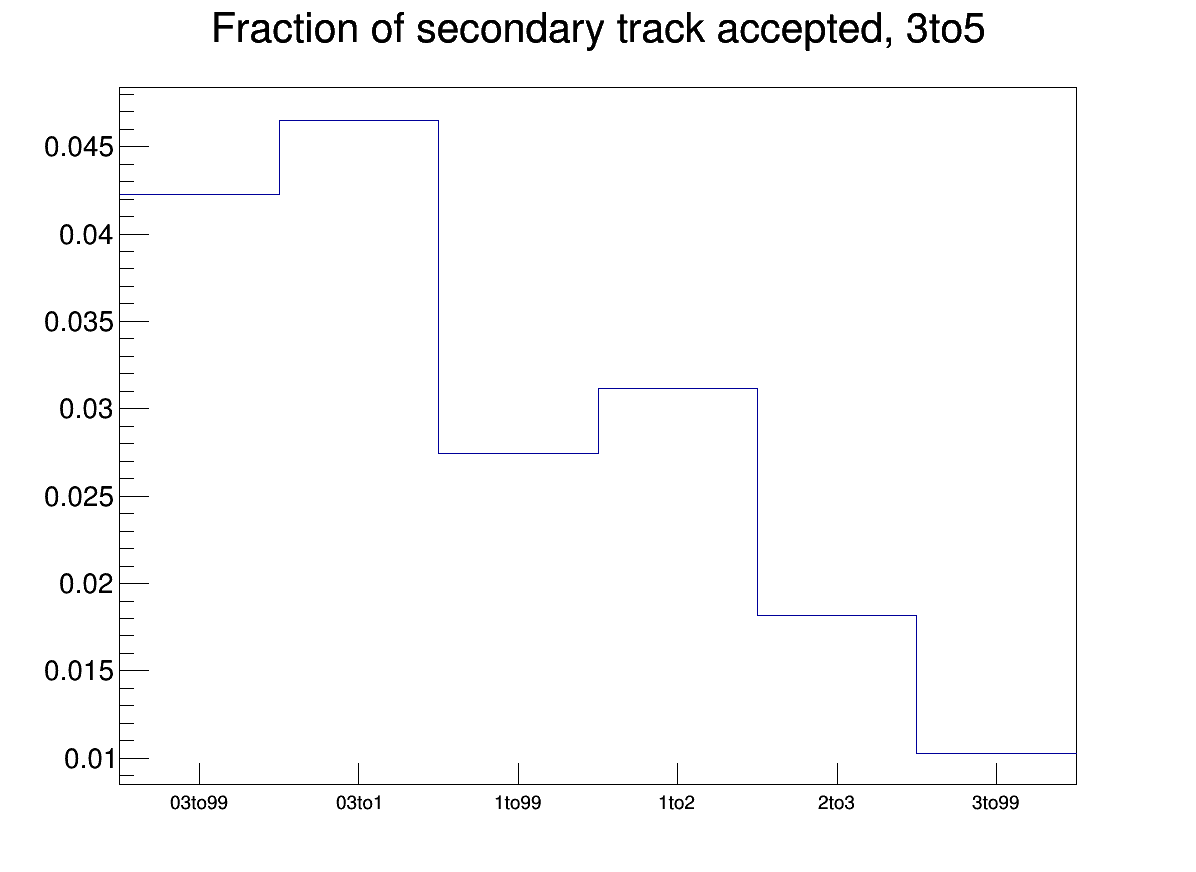
\includegraphics[width=.48\linewidth]{figures/SecTracks/FractOfSecOverTotal_3to5.png}
	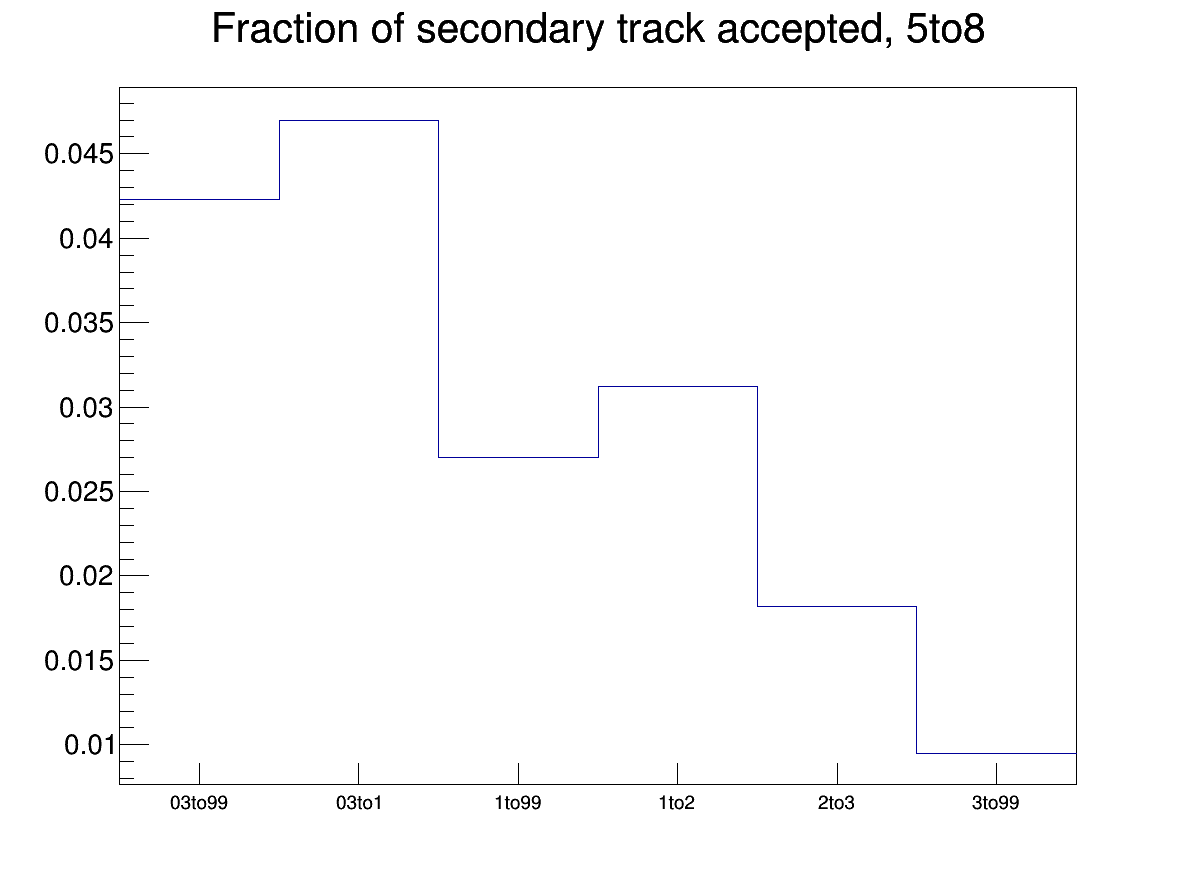
\includegraphics[width=.48\linewidth]{figures/SecTracks/FractOfSecOverTotal_5to8.png}
    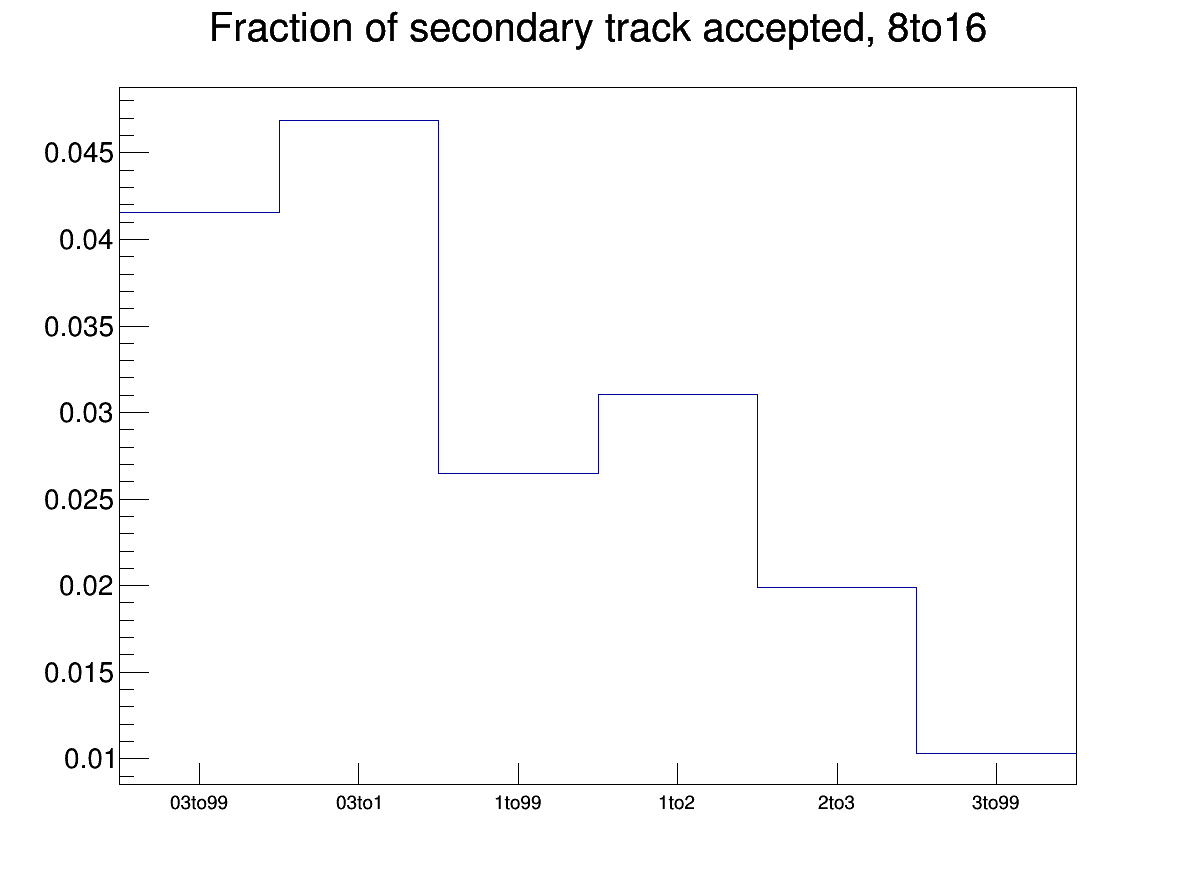
\includegraphics[width=.48\linewidth]{figures/SecTracks/FractOfSecOverTotal_8to16.png}
    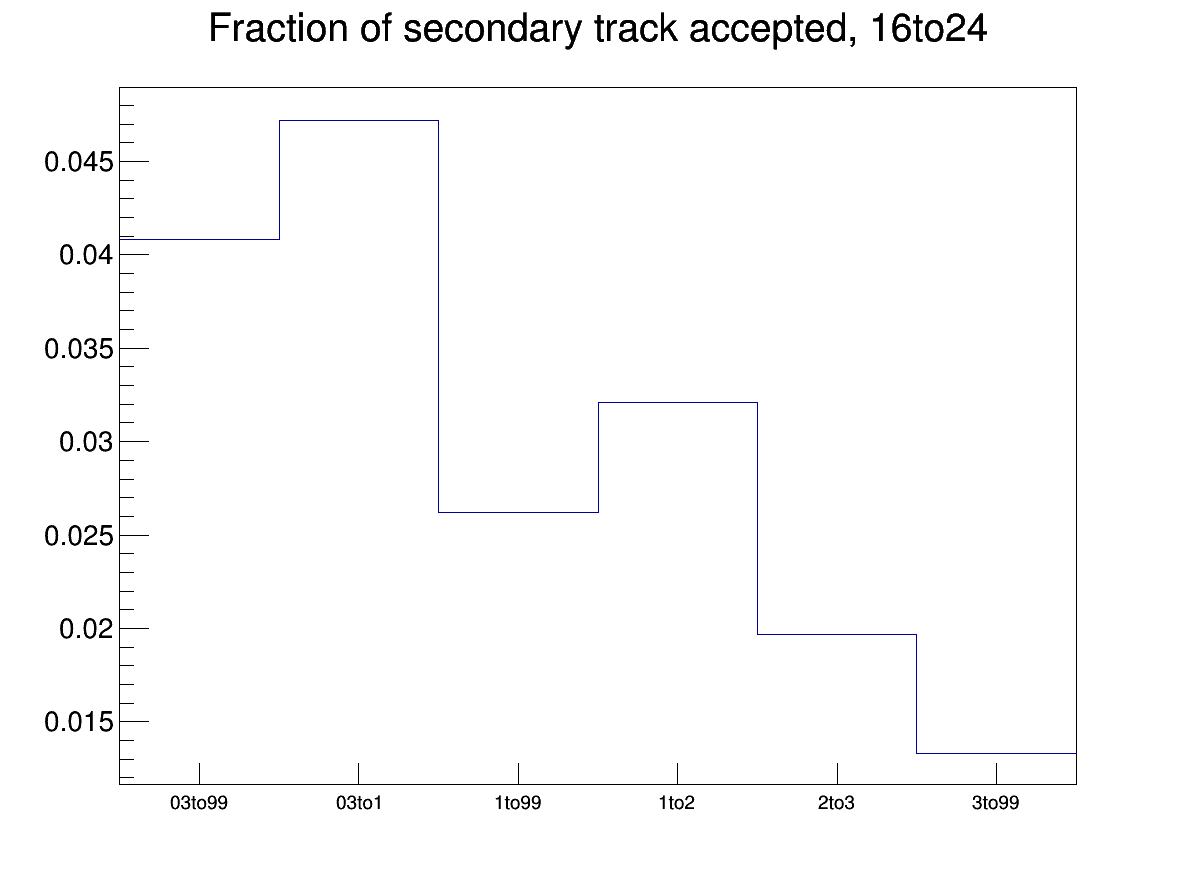
\includegraphics[width=.48\linewidth]{figures/SecTracks/FractOfSecOverTotal_16to24.png}
	\caption{Fraction of secondary tracks over total amount of tracks which pass the DCA selection. The four panel show the fractions for the D-meson $\pt$ ranges: 3-5, 5-8, 8-16, 16-24, respectively. Inside each panel, the associated track $\pt$ ranges are shown on the $x$-axis.}
	\label{fig:secnumber}	
\end{figure}

\begin{figure}[h]   %da B
	\centering
	%Marianna
		  % by Fabio
	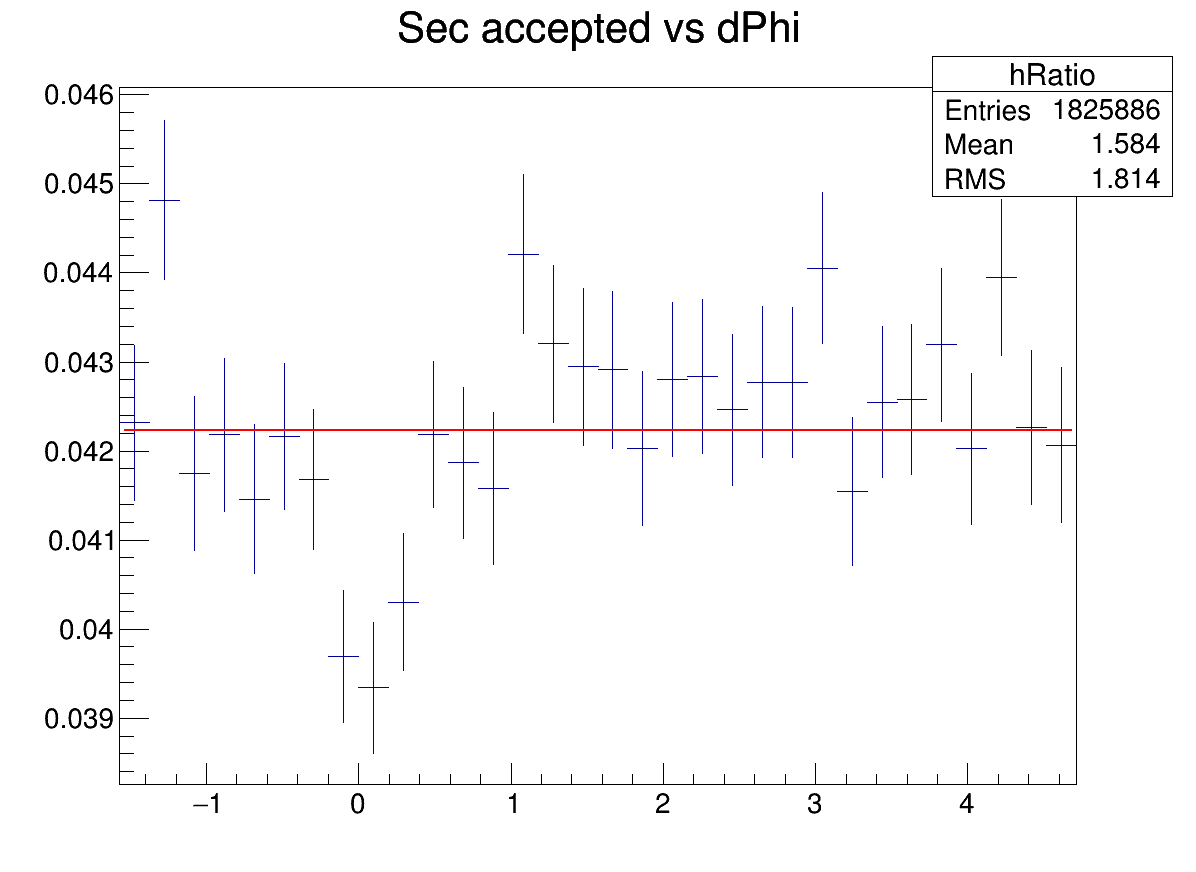
\includegraphics[width=.48\linewidth]{figures/SecTracks/DeltaPhi_3to5_03to99_RatioSecOverAll.png}
	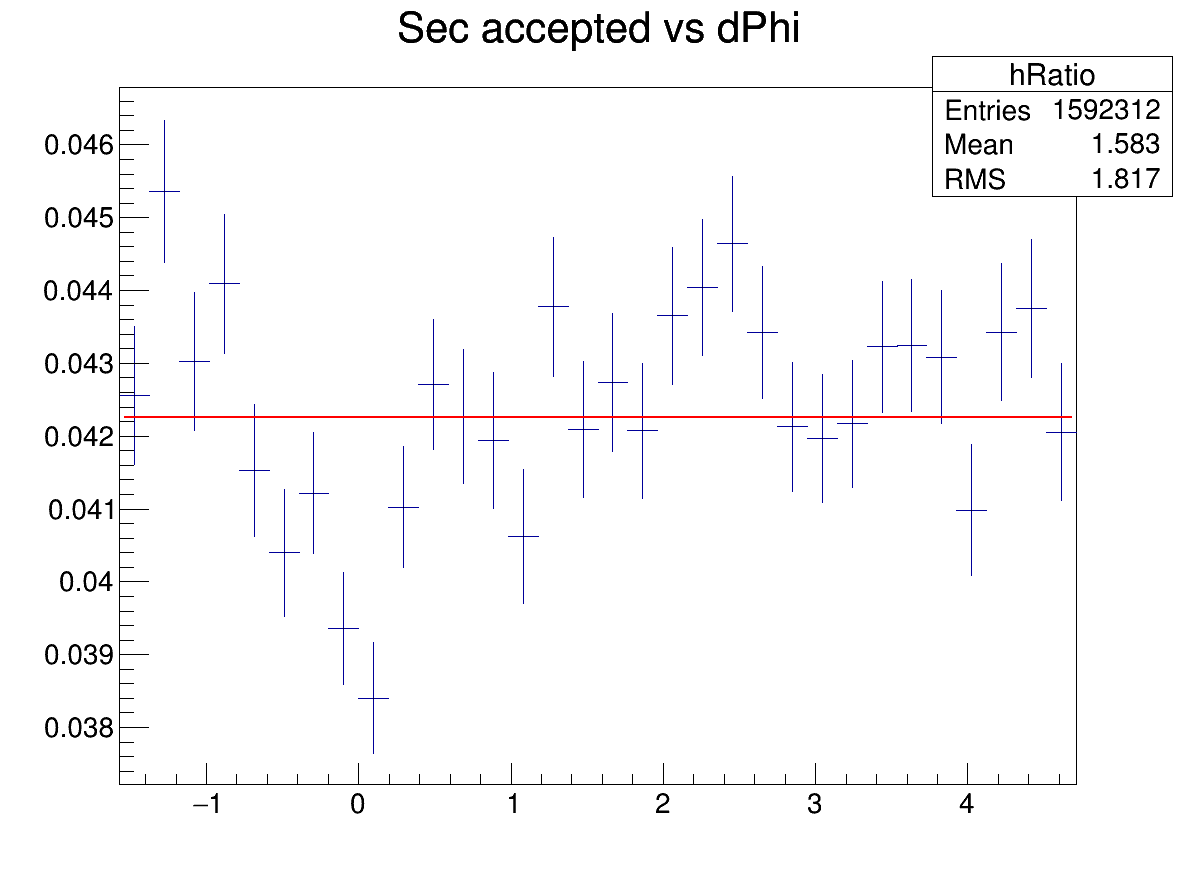
\includegraphics[width=.48\linewidth]{figures/SecTracks/DeltaPhi_5to8_03to99_RatioSecOverAll.png}
    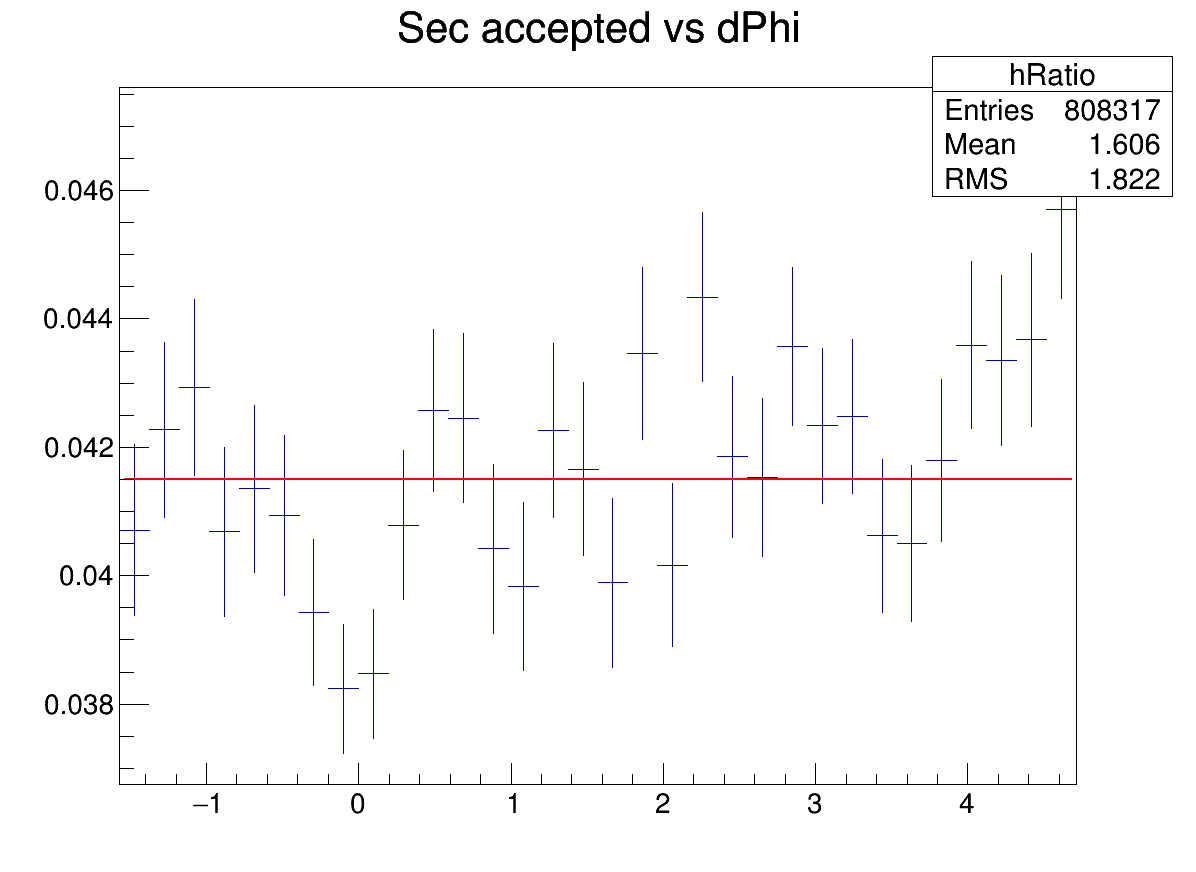
\includegraphics[width=.48\linewidth]{figures/SecTracks/DeltaPhi_8to16_03to99_RatioSecOverAll.png}
    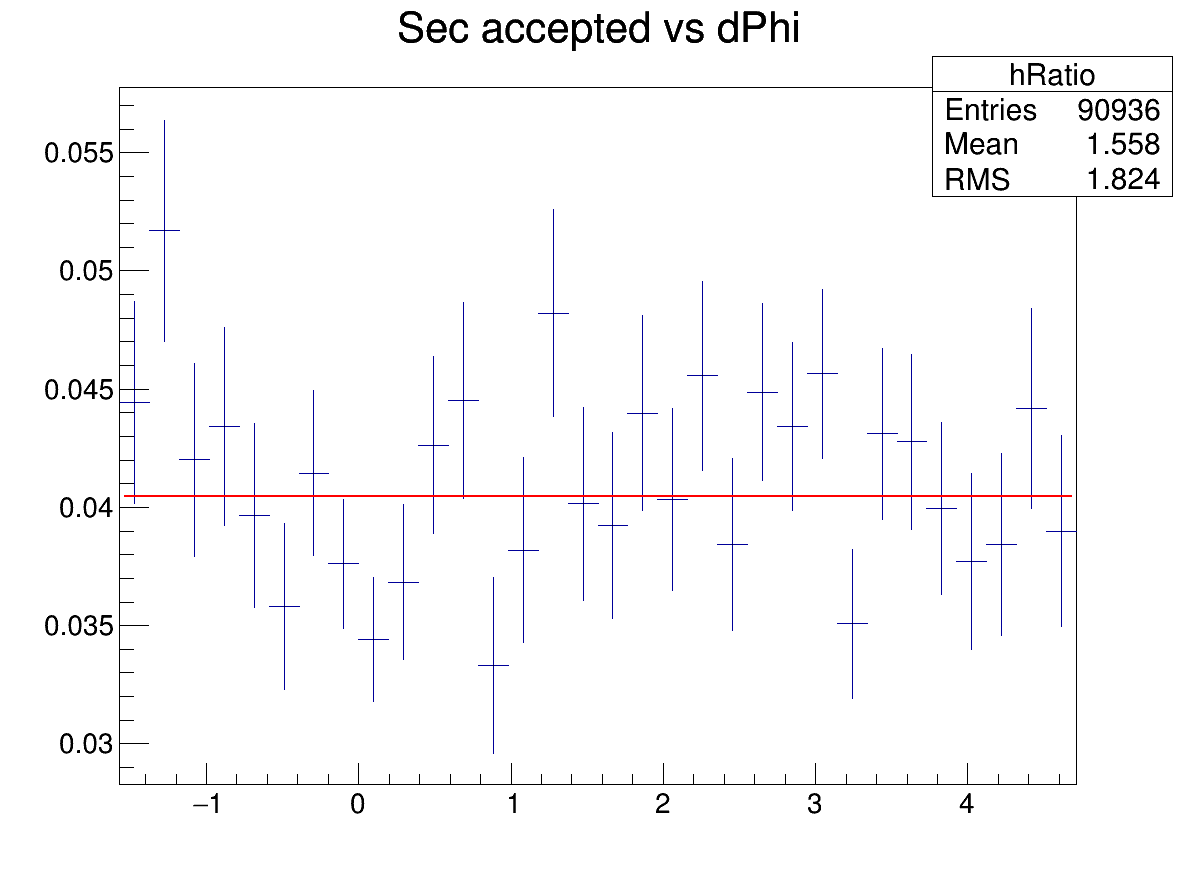
\includegraphics[width=.48\linewidth]{figures/SecTracks/DeltaPhi_16to24_03to99_RatioSecOverAll.png}
	\caption{$\Delta\phi$ dependence of the fraction of secondary tracks in the $\Dzero$-h correlation distributions. The four panel show the fractions for the D-meson $\pt$ ranges: 3-5, 5-8, 8-16, 16-24, respectively. The associated track $\pt$ ranges is the integrated one, i.e. $\pt > 0.3$ GeV/c.}
	\label{fig:secdPhi}	
\end{figure}

It was also verified with the same Monte Carlo study that applying the DCA selection rejects less than 0.2\% primary tracks (tagged as false positives) from the associated track sample, again with a flat azimuthal distribution, inducing hence a fully negligible bias on the data correlation distributions. This is shown in Figure \ref{fig:primRej}. This was also verified for specific charm-origin and beauty-origin tracks, due to their larger DCA with respect to primary tracks from light quarks. In this case, the fraction of rejected charm and beauty tracks stays below 1\% in all the kinematic ranges apart from the associated track $\pt$ regions 0.3-1 and $<0.3$, where the rejection can be as high as 2\%. In these kinematic ranges, though, the data correlation distributions are dominated by non-heavy-flavour tracks, as it was verified from the simulations, hence the overall bias is still contained below 1\%, thus negligible.

\begin{figure}[h]   %da B
	\centering
			  % by Fabio
	\includegraphics[width=.48\linewidth]{figures/SecTracks/FractOfPrimAccepted_3to5.png}
	\includegraphics[width=.48\linewidth]{figures/SecTracks/FractOfPrimAccepted_5to8.png}
    \includegraphics[width=.48\linewidth]{figures/SecTracks/FractOfPrimAccepted_8to16.png}
    \includegraphics[width=.48\linewidth]{figures/SecTracks/FractOfPrimAccepted_16to24.png}
	\caption{Fraction of primary tracks rejected by the DCA selection. The four panel show the fractions for the D-meson $\pt$ ranges: 3-5, 5-8, 8-16, 16-24, respectively. Inside each panel, the associated track $\pt$ ranges are shown on the $x$-axis.}
		\label{fig:primRej}	
\end{figure}

These studies were performed on an enriched Monte Carlo sample, which could not fully reproduce the relative abundancies of the species. Anyway, for events with a reconstructed D-meson, this bias is expected to be minor, and only these events are used in the data analysis. In any case, the percentages obtained from the study were found to be consistent within 1\% with the outcome of the studies for the p-Pb 2013 analysis, which reassures us on the full validity of these results.

\clearpage
%\end{document}
